% vim: tw=0:wrap:linebreak
\documentclass[12pt]{article}

% \setcitestyle{numbers}
\usepackage[numbers]{natbib}
\usepackage[english]{babel}
\usepackage[utf8x]{inputenc}
\usepackage{amsmath}
\usepackage{graphicx}
\usepackage{longtable}
\usepackage[]{hyperref}
\usepackage{comment}
\usepackage{xspace}
\usepackage[usenames]{color} 
\usepackage{datetime}
\usepackage{microtype}

\newcommand{\vstretch}[1]{\vspace*{\stretch{#1}}}
\newcommand{\code}[1]{\texttt{#1}}

\newcommand{\DIASource}{\code{DIASource}\xspace}
\newcommand{\DIASources}{\code{DIASources}\xspace}
\newcommand{\DIAObject}{\code{DIAObject}\xspace}
\newcommand{\DIAObjects}{\code{DIAObjects}\xspace}
\newcommand{\DB}{{Level 1 database}\xspace}
\newcommand{\DR}{{Level 2 database}\xspace}
\newcommand{\Object}{\code{Object}\xspace}
\newcommand{\Objects}{\code{Objects}\xspace}
\newcommand{\Source}{\code{Source}\xspace}
\newcommand{\Sources}{\code{Sources}\xspace}
\newcommand{\ForcedSource}{\code{ForcedSource}\xspace}
\newcommand{\ForcedSources}{\code{ForcedSources}\xspace}
\newcommand{\CoaddSource}{\code{CoaddSource}\xspace}
\newcommand{\CoaddSources}{\code{CoaddSources}\xspace}
\newcommand{\SSObject}{\code{SSObject}\xspace}
\newcommand{\SSObjects}{\code{SSObjects}\xspace}
\newcommand{\VOEvent}{\code{VOEvent}\xspace}
\newcommand{\VOEvents}{\code{VOEvents}\xspace}
\newcommand{\transSNR}{5\xspace}

% Command to link to a document in Docushare. Pass an LSST document handle as argument, or a document number
\newcommand{\ds}[2]{{\color{blue} \href{https://docushare.lsstcorp.org/docushare/dsweb/Get/#1}{#2}}\xspace}

\newcommand{\SRD}{\ds{LPM-17}{SRD}}
\newcommand{\DPDD}{\ds{LSE-163}{DPDD}}
\newcommand{\LSR}{\ds{LSE-29}{LSR}}
\newcommand{\OSS}{\ds{LSE-30}{OSS}}
\newcommand{\DMSR}{\ds{LSE-61}{DMSR}}
\newcommand{\appsUMLdomain}{\ds{LDM-133}{LDM-133}}
\newcommand{\appsUMLusecase}{\ds{LDM-134}{LDM-134}}
\newcommand{\SUI}{\ds{LDM-131}{SUID}}
\newcommand{\DMSD}{\ds{LDM-148}{DMSD}}
\newcommand{\MOPSD}{\ds{LDM-156}{MOPSD}}
\newcommand{\DMMD}{\ds{LDM-152}{DMMD}}
\newcommand{\DMOps}{\ds{LDM-230}{DM OpsCon}}
\newcommand{\SDQAP}{\ds{LSE-63}{LSE-63}}
\newcommand{\NewPCP}{\ds{LSE-180}{LSE-180}}
\newcommand{\UCAL}{\ds{Document-15125}{UCAL}}

\newcommand{\wbsSFM}{WBS 02C.03.01}
\newcommand{\wbsAssocP}{WBS 02C.03.02}
\newcommand{\wbsAP}{WBS 02C.03.03}
\newcommand{\wbsDiffim}{WBS 02C.03.04}
\newcommand{\wbsMOPS}{WBS 02C.03.06}
\newcommand{\wbsSDQAP}{WBS 02C.01.02.02}
\newcommand{\wbsSDQAT}{WBS 02C.01.02.02}
\newcommand{\wbsSPT}{WBS 02C.01.02.03}
\newcommand{\wbsPSF}{WBS 02C.04.03}
\newcommand{\wbsCoadd}{WBS 02C.04.04}
\newcommand{\wbsDetDeblend}{WBS 02C.04.05}
\newcommand{\wbsObjChar}{WBS 02C.04.06}
\newcommand{\wbsAFW}{WBS 02C.03.05, 02C.04.01}
\newcommand{\wbsCPP}{WBS 02C.04.02}
\newcommand{\wbsPhotoCal}{WBS 02C.03.07}
\newcommand{\wbsAstroCal}{WBS 02C.03.08}

\newenvironment{note}[1][Note]
{
  \begin{displaymath}
    \left[ \qquad
    \begin{minipage}[h]{.75\linewidth}
      \color{red} \footnotesize
      \textbf{#1:} \newline
      \color{black}
}
{
    \end{minipage}
    \normalsize
    \qquad \right]
  \end{displaymath}
}

\newcommand{\uc}[1]{{\tt #1}}

\setcounter{secnumdepth}{5}
\setcounter{tocdepth}{5}

\title{Large Synoptic Survey Telescope \\
Data Management Applications Design \\
{\author{
    Mario Juri\'c\footnote{Please direct comments to \textless\href{mailto:mjuric@lsst.org}{mjuric@lsst.org}\textgreater.},
    R.H. Lupton, T. Axelrod, J.F. Bosch, P.A. Price, \\
    G.P. Dubois-Felsmann, \v{Z}. Ivezi\'c, A.C. Becker, J. Becla,  \\ 
     A.J. Connolly, J. Kantor, K-T Lim, D. Shaw, \\
    {\em for the LSST Data Management}
}}}

\begin{document}
\date{\today, \currenttime hrs}
\maketitle
\pagestyle{headings}

\begin{abstract}
The LSST Science Requirements Document (the LSST \SRD) specifies a set of
data product guidelines, designed to support science goals envisioned to be enabled by the LSST observing program. Following these guidlines, the details of these data products have been described in the LSST Data Products Definition Document (\DPDD), and captured in a formal flow-down from the \SRD via the LSST System Requirements (\LSR), Observatory System Specifications (\OSS), to the Data Management System Requirements (\DMSR).
The LSST Data Management subsystem's responsibilities include the design, implementation, deployment and execution of software pipelines necessary to generate these data products. This document, in conjunction with the UML Use Case model (\appsUMLusecase), describes the design of the scientific aspects of those pipelines.
\end{abstract}


\tableofcontents

\include{sections/preface}

\section{Introduction}

\subsection{LSST Data Management System}

To carry out this mission the Data Management System (DMS) performs the following major functions:

\begin{itemize}
\item Processes the incoming stream of images generated by the camera
  system during observing to produce transient alerts and to archive
  the raw images.

\item Roughly once per year, creates and archives a Data Release (``DR''),
  which is a static self-consistent collection of data products
  generated from all survey data taken from the date of survey
  initiation to the cutoff date for the Data Release. The data
  products (described in detail in the \DPDD), include measurements of 
  the properties (shapes, positions, fluxes, motions, etc.) of all detected
  objects, including those below the single visit sensitivity limit,
  astrometric and photometric calibration of the full survey object
  catalog, and limited classification of objects based on both their
  static properties and time-dependent behavior.  Deep coadded images
  of the full survey area are produced as well.

\item Periodically creates new calibration data products, such as bias
  frames and flat fields, that will be used by the other processing
  functions, as necessary to enable the creation of the data products above.

\item Makes all LSST data available through interfaces that utilize,
  to the maximum possible extent, community-based standards such as those
  being developed by the Virtual Observatory (``VO''), and facilitates user
  data analysis and the production of user-defined data products at Data
  Access Centers (``DAC'') and at external sites.
\end{itemize}

The overall architecture of the DMS is discussed in more detail in the Data Management System Design (\DMSD) document. The overall architecture of the DMS is shown in Figure~\ref{fig:DMS}.
\\

This document discusses the role of the Applications layer in the first three functions listed above (the functions involving \emph{science pipelines}).  The fourth is discussed separately in the SUI Conceptual Design Document (\SUI).

\begin{figure}
\centering
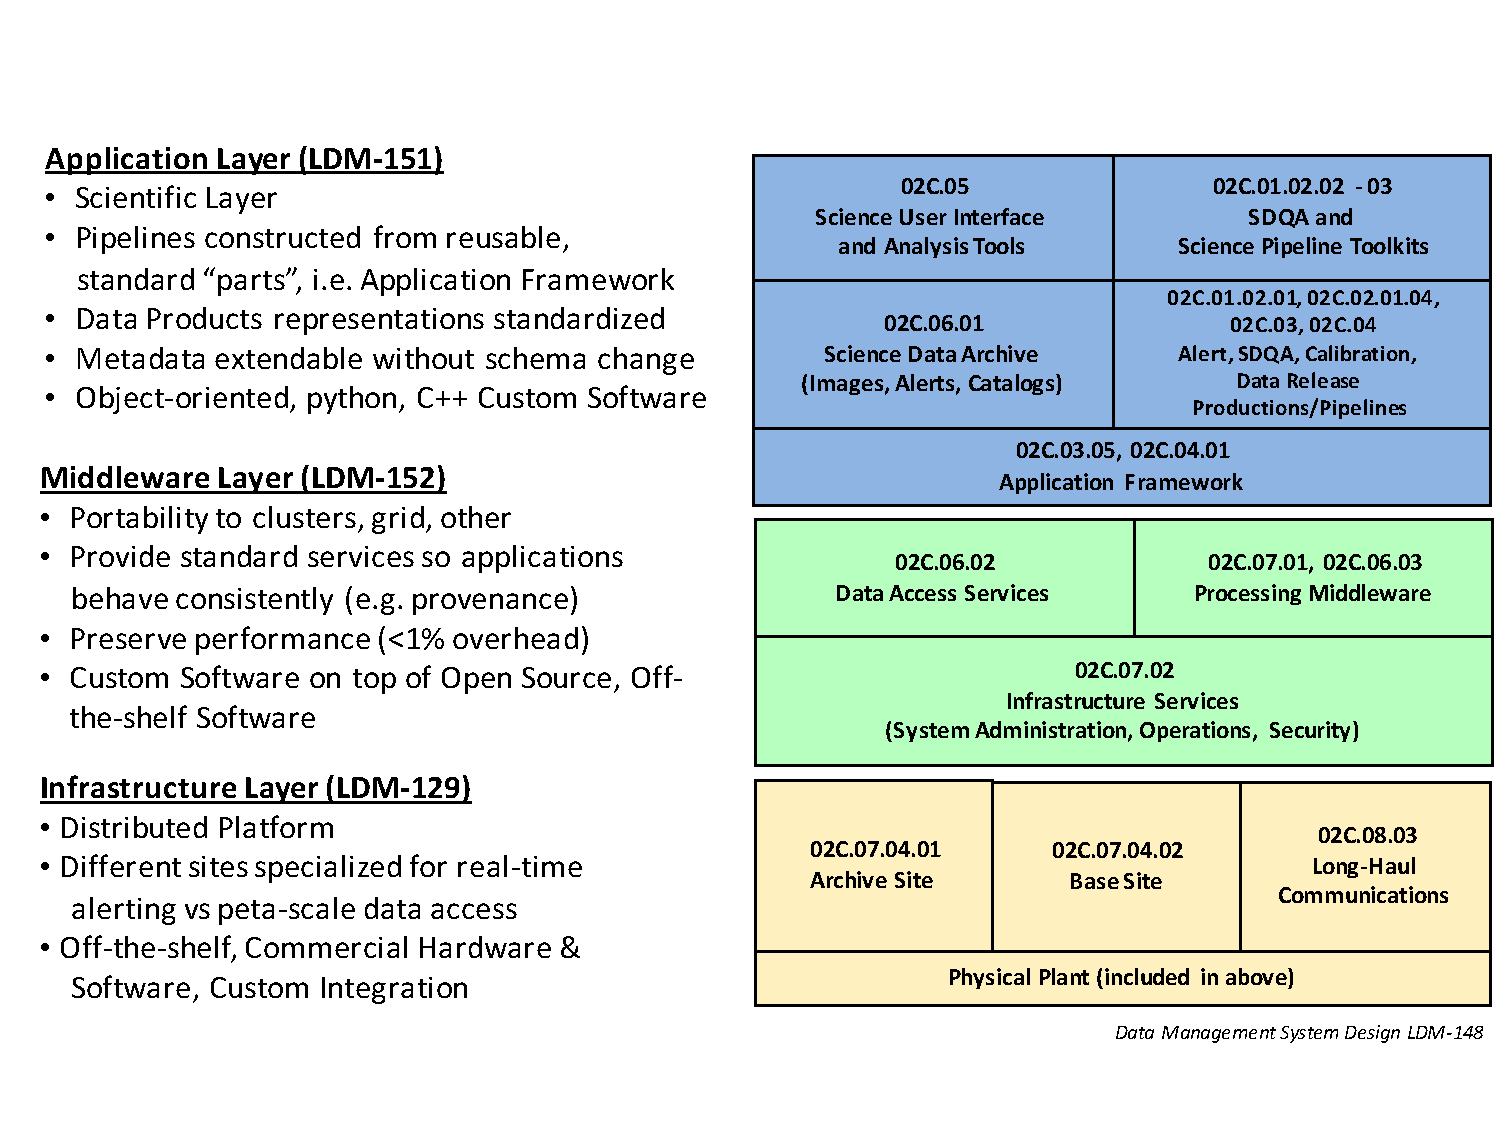
\includegraphics[angle=90,scale=0.70]{figures/DMS-Architecture.pdf}
\caption{Architecture of the Data Management System\label{fig:DMS}}
\end{figure}

\begin{figure}
%\includegraphics[angle=90,scale=0.70]{ApplicationLayerProductionsandPipelines.eps}
\centering
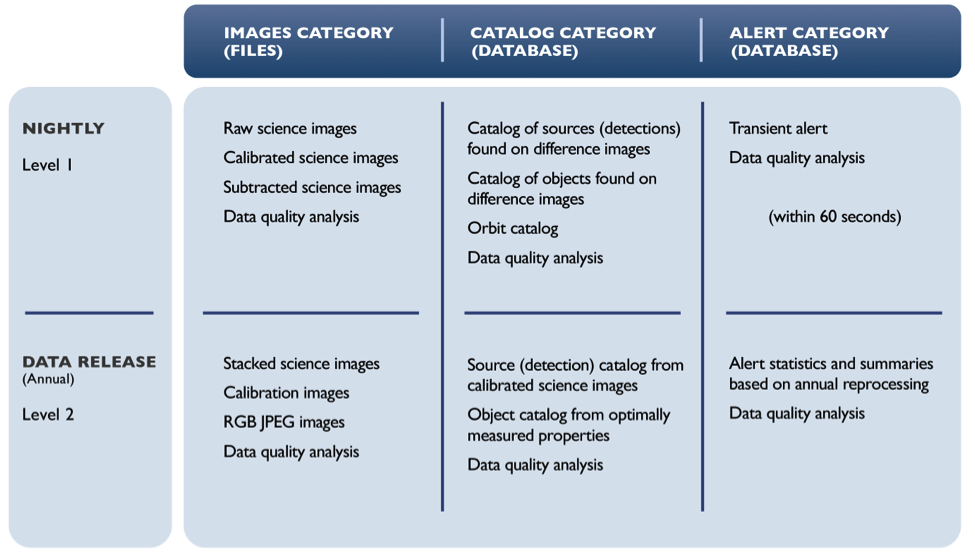
\includegraphics[angle=90]{figures/DataProductDelivarables.png}
\caption{Organization of LSST Data Products\label{fig:DP}}
\end{figure}

\subsection{Data Products}

The LSST data products are organized into three groups, based on their intended use and/or origin. The full description is provided in the Data Products Definition Document (\DPDD); we summarize the key properties here to provide the necessary context for the discussion to follow. 

\begin{itemize}
\item {\bf Level 1} products are intended to support timely detection and follow-up
  of time-domain events (variable and transient sources). They are generated by
  near-real-time processing the stream of data from the camera system during 
  normal observing.  Level 1 products are therefore continuously generated and / or
  updated every observing night. This process is of necessity highly
  automated, and must proceed with absolutely minimal human
  interaction.  In addition to science data products, a number of related
  Level 1 ``SDQA''\footnote{Science Data Quality Analysis} data products are generated
  to assess quality and to provide feedback to the Observatory Control System (OCS).

\item {\bf Level 2} products are generated as part of a Data Release, generally
  performed 
  yearly, with an additional data release for the first 6 months of survey data. 
  Level 2 includes data products for which extensive
  computation is required, often because they combine information from
  many exposures.  Although the steps that generate Level 2 products
  will be automated, significant human interaction may be required at
  key points to ensure the quality of the data.

\item {\bf Level 3} products are generated on any computing resources
  anywhere and then stored in an LSST Data Access Center. Often, but not
  necessarily, they will be generated by users of LSST using LSST software
  and/or hardware. LSST DM is required to facilitate the creation of
  Level 3 data products by providing suitable APIs, software components, and
  computing infrastructure, but will not by itself create any Level 3
  data products. Once created, Level 3 data products may be associated with
  Level 1 and Level 2 data products through database federation.
  Where appropriate, the LSST Project, with the agreement of the Level 3
  creators, may incorporate user-contributed Level 3 data product pipelines
  into the DMS production flow, thereby promoting them to Level 1 or 2.

\end{itemize}
%
The organization of LSST Data Products is shown in Figure~\ref{fig:DP}.

Level 1 and Level 2 data products that have passed quality control
tests will be accessible to the public without restriction.
Additionally, the source code used to generate them will be made
available, and LSST will provide support for builds on selected
platforms.

\subsection{Science Pipelines Overview}

We recognize four major groups of science pipelines residing in the Applications layer:
\begin{itemize}
    \item {\bf Level 1 Pipelines}, grouped under the {\bf Alert Production} element of the WBS, are designed to generate Level 1 data products. These include:
    \begin{itemize}
    \item {\bf \emph{Single Frame Processing (``SFM'') Pipeline}} (\wbsSFM), to reduce acquired visits and detect and characterize astrophysical sources present in these visits.
    \item {\bf \emph{Image Differencing Pipeline}} (\wbsDiffim), to create difference images, and detect and characterize sources in them.
    \item {\bf \emph{Association Pipeline}} (\wbsAssocP), to associate sources detected in the difference images with known objects.
    \item {\bf \emph{Alert Generation Pipeline}} (\wbsAP), to generate and transmit alerts to time-domain events (e.g., transients) to the astronomical community, and
    \item {\bf \emph{Moving Object Pipeline}} (\wbsMOPS), to identify, link and compute orbits for Solar System objects detected in difference images.
    \end{itemize}
Level 1 pipelines run as the data are being acquired. They primarily focus on image differencing, and the reduction of information extracted from difference images. The algorithms they employ are designed and chosen to complete processing on minute (alert production) to day (\textbf{\emph{DayMOPS}}) time scales. They are also rerun as a part of Data Release Production (DRP), potentially in somewhat different configurations to achieve greater precision at the expense of increased runtime.
    
    \item {\bf Level 2 Pipelines} run annually or semi-annualy (for the first year of data), and are designed to generate deep co-adds and catalogs stemming from analysis of direct image data.  These include:
    \begin{itemize}
        \item {\bf \emph{PSF Estimation Pipeline}} (\wbsPSF), to estimate the PSF properties and variation across the focal plane for each visit, to the degree of precision required by the \SRD. Note that the work of this pipeline goes beyond the typical single-CCD PSF estimation present in the SFM pipeline.
        \item {\bf \emph{Image Coaddition Pipeline}} (\wbsCoadd), to generate and characterize coadded images of the sky, as well as create templates for image differencing.
        \item {\bf \emph{Object Detection and Deblending}} (\wbsDetDeblend), to detect sources in images of the sky and decompose them into individual astronomical objects.
        \item {\bf \emph{Object Characterization Pipeline}} (\wbsObjChar), to characterize (perform measurements of) astrophysical objects detected in LSST imaging (both in single frames and coadds).
    \end{itemize}
    
    \item {\bf Calibration Pipelines} process the collected calibration data and perform calibration of LSST instruments and data products. These include:
    \begin{itemize}
        \item {\bf \emph{Calibration Products Pipeline}} (\wbsCPP), that generates the necessary calibration data products (e.g., master flats, biases, atmospheric models, etc.). It is run periodically as new calibration data are acquired.
        \item {\bf \emph{Photometric Calibration Pipeline}} (\wbsPhotoCal), that performs global photometric self-calibration of the Level 2 dataset.
        \item {\bf \emph{Astrometric Calibration Pipeline}} (\wbsAstroCal), that performs global astrometric self-calibration of the Level 2 dataset.
    \end{itemize}
    The calibration products pipeline is also rerun as a part of Data Release Processing. Global self-calibration steps run in DRP only.

       \item {\bf Science Data Quality Assessment (SDQA) pipelines and toolkits}, to enable collection, computation, visualization, monitoring and analysis of data quality metrics across all pipelines. These are divided into:
       \begin{itemize}
           \item {\bf \emph{Science Data Quality Assessment Pipeline}} (\wbsSDQAP), that provides low-level data collection functionality for SDQA and
           \item {\bf \emph{Science Data Quality Analyst Toolkit}} (\wbsSDQAT), that provides the visualization, analysis and monitoring capabilities for SDQA.
       \end{itemize}

\end{itemize}

In addition to these four, we recognize two other, cross-cutting, elements of DMS functionality:

\begin{itemize}
       \item {\bf \emph{Common Image and Catalog Processing Framework}} (\wbsAFW), known as the {\bf Application Framework (afw)}, that collects base classes and algorithms % RHL need a better word than algorithms
         used by the DM Applications layer. The framework is split in two WBS elements, to reflect the multi-institutional nature of the work, but is functionally viewed as a single, integrated, component (class library).
       \item The {\bf \emph{Science Pipeline Toolkit}} (\wbsSPT), a collection of software components (and design principles) designed to enable construction of Level 3 pipelines relying on reusable lower-level components produced in support of other LSST DM software.
\end{itemize}

\subsubsection{Level 1 Pipelines Overview}
The production of Level 1 products is generally performed nightly, directly fed by 
the output data stream from the Camera SDS\footnote{Science Array Data Acquisition (DAQ) Subsystem} during observing. This data stream
contains both unprocessed (raw) camera images, and images that have been corrected
for crosstalk by the SDS on the Summit.  The normal observing
pattern is to take two 15 second exposures of the same field in immediate
succession.  These two exposures together form a {\em visit}, which is the typical
image data unit processed by the rest of the DM system.
\\

\begin{figure}
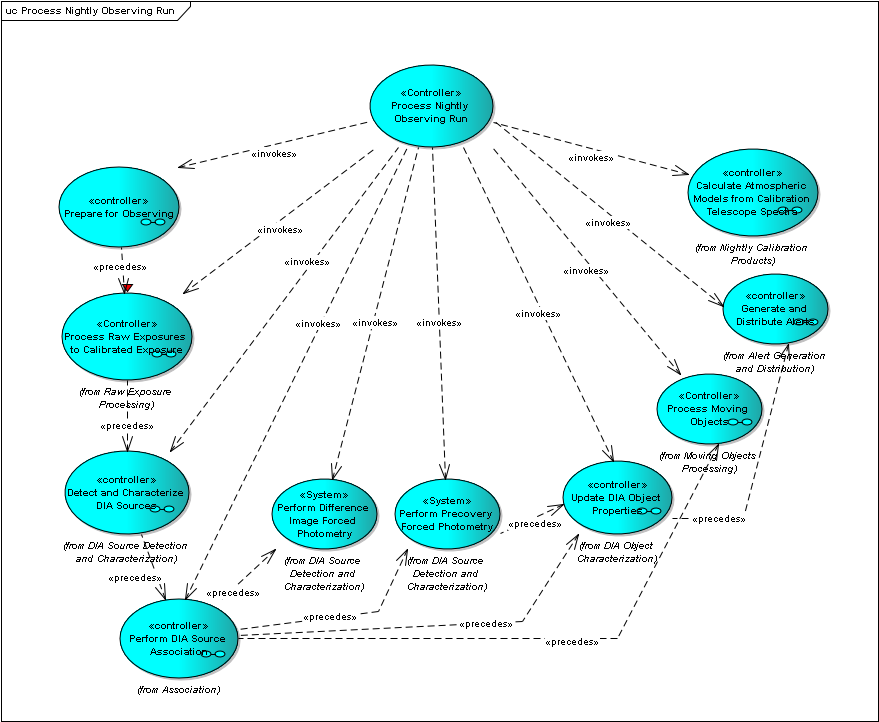
\includegraphics[angle=0,scale=0.44]{figures/process_nightly_observing_run.png}
\caption{Level 1 Processing Flow Diagram\label{fig:level1}}
\end{figure}

The logical flow of Level 1 processing is shown in the Use Case diagram presented in Figure~\ref{fig:level1}. For every observation, the following sequence of events will unfold:
%
\begin{enumerate}
\item A visit is acquired (\uc{Prepare for Observing}) and reduced (\uc{Process Raw Exposures to Calibrated Exposure}) to a single {\em visit image}. This includes instrumental signature removal\footnote{E.g., subtraction of bias and dark frames, flat fielding, bad pixel/column interpolation, etc.}, combining of snaps, etc.
  % RHL I removed cosmic ray rejection as it's not clear if it's in ISR or snap combination.

\item The visit image is differenced against the appropriate template and \DIASources are detected (\uc{Detect and Characterize DIA Sources}). If necessary, deblending is performed at this stage.

The flux and shape of the DIASource are measured on the difference image. PSF photometry is performed on the visit image at the position of the \DIASource to obtain a measure of the absolute flux.
  % RHL this is tricky in crowded fields (inc. SNe on galaxies).  We should rethink this a bit at some point.

\item The \DB is searched for a \DIAObject or an \SSObject with which to positionally associate the newly discovered \DIASource. If no match is found, a new \DIAObject is created and the observed \DIASource is associated to it.

If the \DIASource has been associated to an \SSObject (a known Solar System object), it will be flagged as such and an alert will be issued. Further processing will occur in daytime (\uc{Process Moving Objects}).

\item Otherwise, the associated \DIAObject measurements will be updated with new data (\uc{Update DIA Object Properties}). All affected columns will be recomputed, including proper motions, centroids, light curves, nearest Level 2 \Objects, etc.
  % RHL do we really want to update e.g. the proper motion/parallax on each visit?

\item An alert is issued (\uc{Generate and Distribute Alerts}) that includes all required components, as described in the \DPDD.

\item For all \DIAObjects overlapping the field of view to which a \DIASource from this visit has \emph{not} been associated, forced photometry will be performed (\uc{Perform Difference Image Forced Photometry}).  No alerts will be issued for these measurements.

\end{enumerate}

Within 24 hours of discovery, LSST DM system will perform \emph{precovery} PSF forced photometry on any prior difference image overlapping the predicted position of new \DIAObjects taken within the past 30 days (\uc{Perform Precovery Forced Photometry}).
\\

Similarly, in daytime after the nightly observing run, atmospheric models from the calibration telescope spectra will be calculated (\uc{Calculate Atmospheric Models from Calibration Telescope Spectra}) and made available to the users.
\\

In addition to these, the Moving Object Pipeline (MOPS; \wbsMOPS; \uc{Process Moving Objects}) will also be run in daytime. It is described in its own section of this document, with a detailed design in a separate Moving Object Pipeline Design Document (\MOPSD).

\subsubsection{Level 2 Pipelines Overview}

\begin{figure}[!htbp]
    \centering
    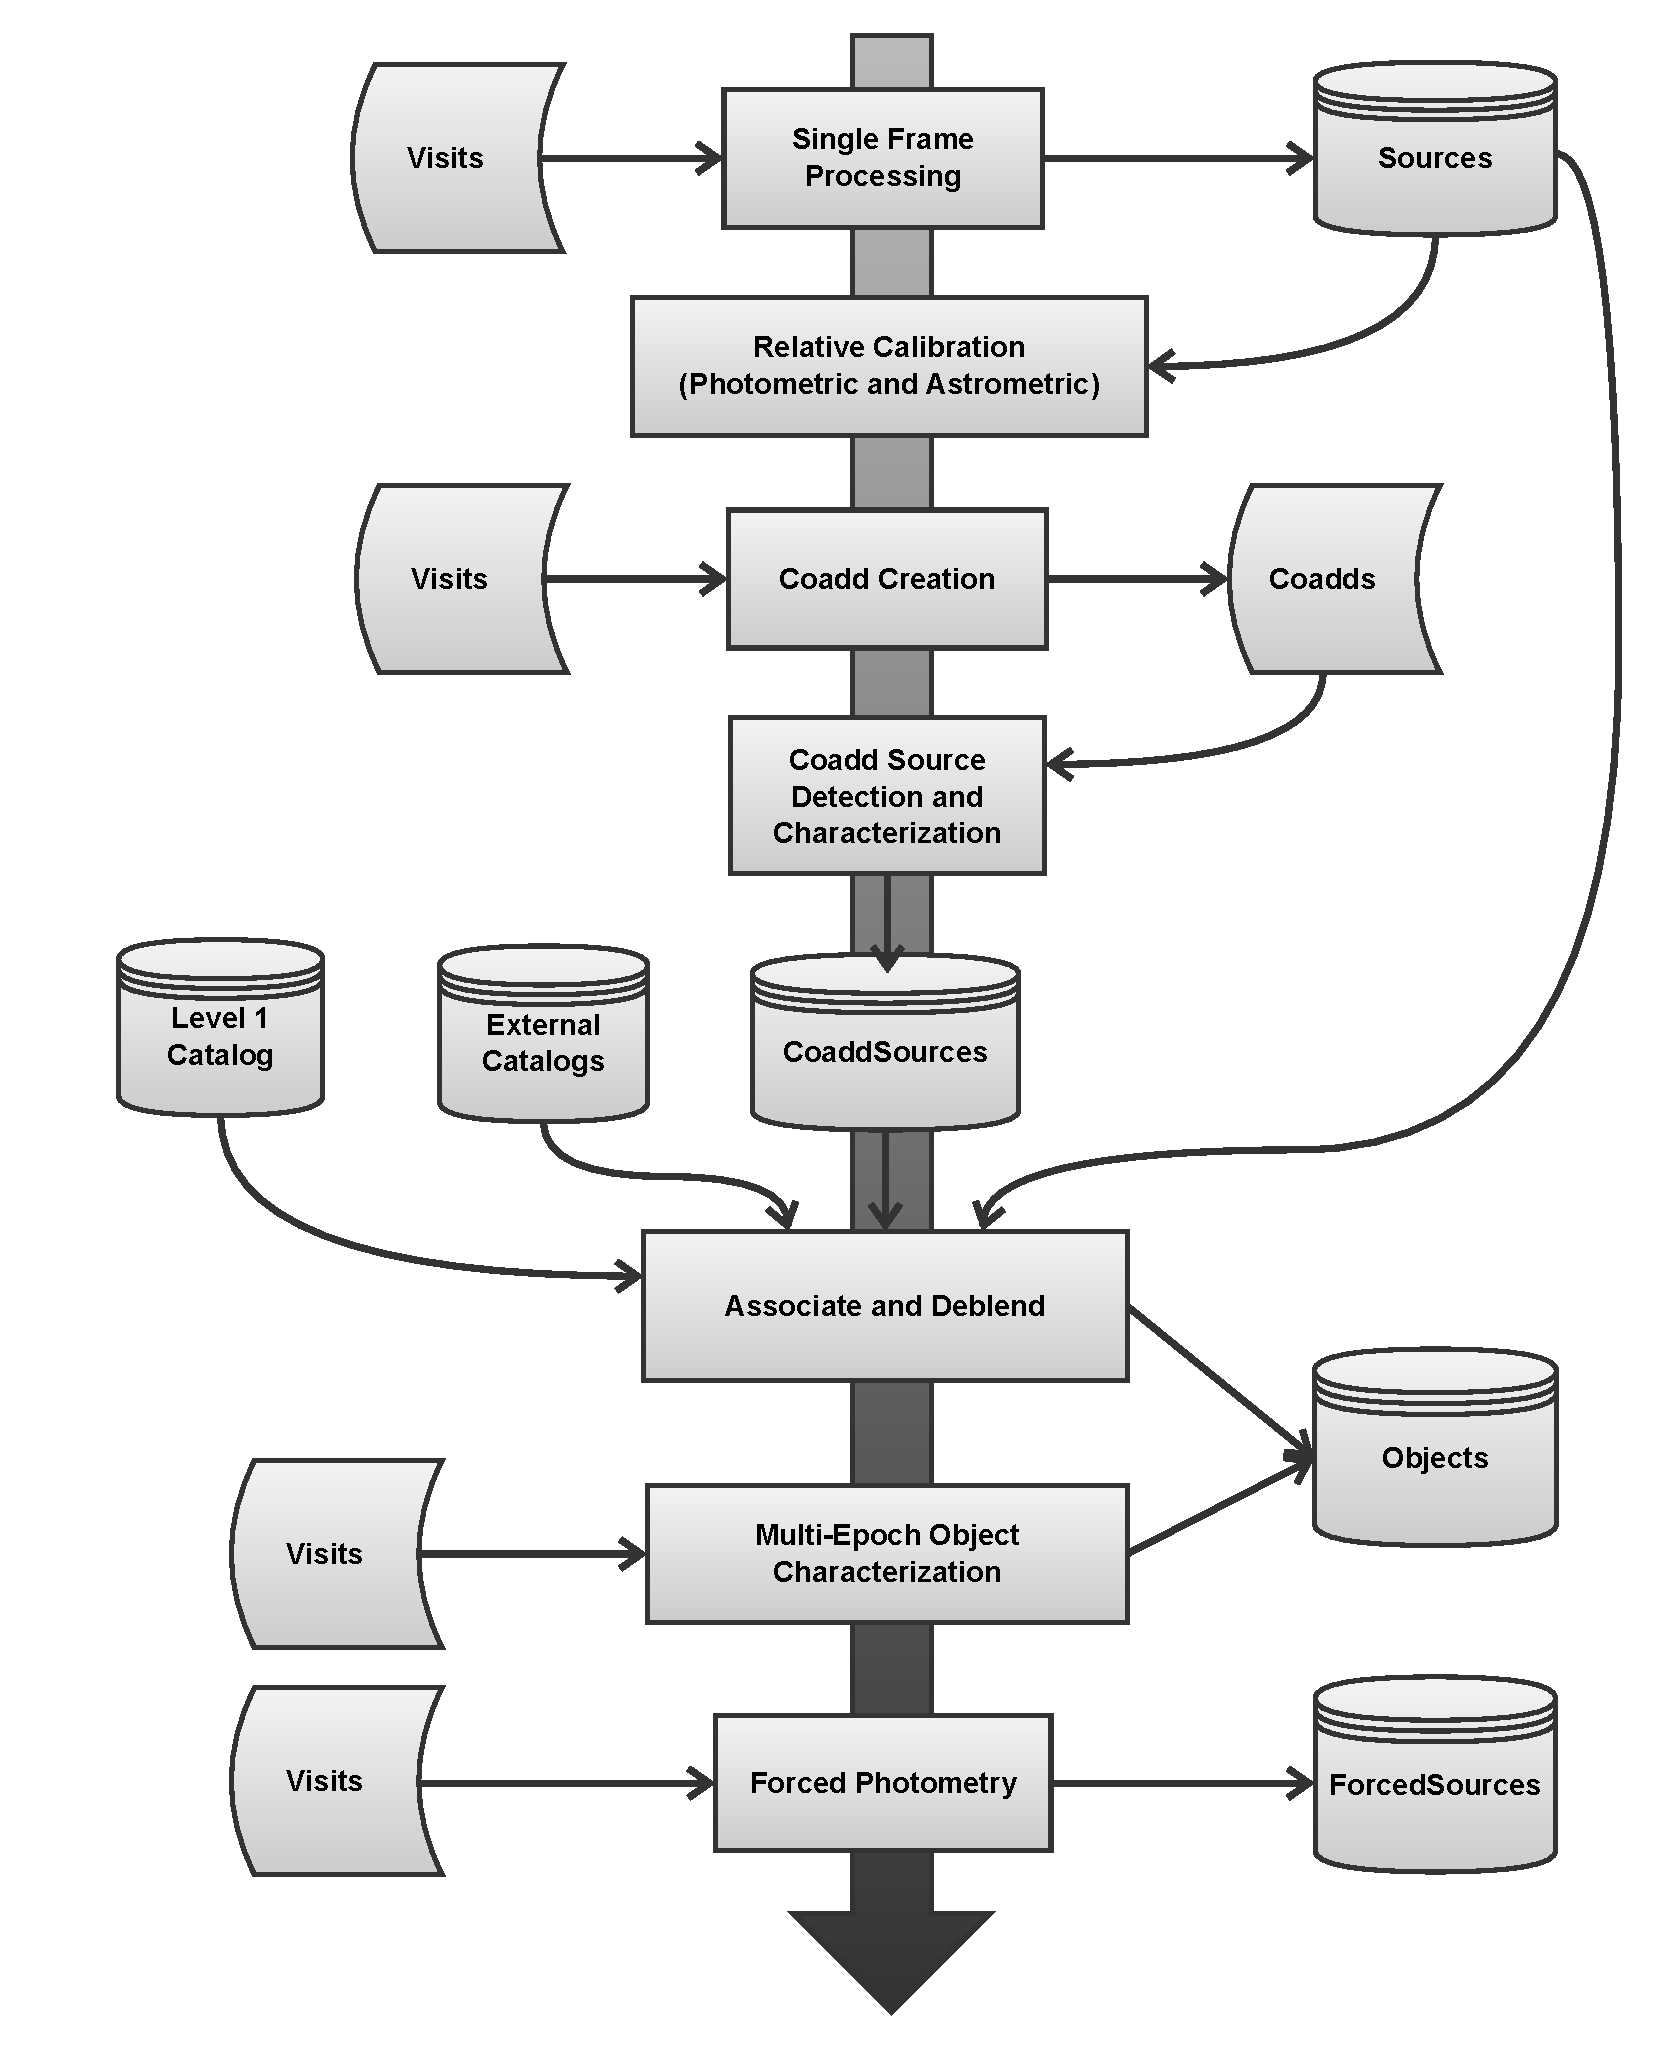
\includegraphics[scale=0.5]{figures/Level_2_Processing_Flowchart}
    \caption{Level 2 Processing Overview\label{fig:level2dp}}    
\end{figure}

Figure~\ref{fig:level2dp} presents a high-level overview of the Level 2 data processing workflow. Logically\footnote{The actual implementation may parallelize these steps to the extent possible; see LDM-230, the Automated DM Operations Document (\DMOps).}, the processing begins with single-frame (visit) image reduction and source measurement, followed by global astrometric and photometric calibration, coadd creation, detection on coadds, association and deblending, object characterization, and forced photometry measurements. The UML Use Case model (\appsUMLusecase) captures these activities in the \uc{Produce a Data Release} diagram.
\\

The following is a high-level description of steps which occur during regular Level 2 data processing:
\begin{enumerate}
    \item \emph{Single Frame Processing}: Raw exposures are reduced to \emph{calibrated visit exposures}, and \Sources are independently detected, deblended, and measured on all visits. Their measurements (instrumental fluxes and shapes) are stored in the \Source table. This step is performed by the {\bf \emph{Single Frame Processing Pipeline}} (\wbsSFM).
    \item \emph{Relative calibration}: The survey is internally calibrated, both photometrically and astrometrically using the {\bf \emph{Astrometric}} (\wbsAstroCal) and {\bf \emph{Photometric Calibration Pipelines}} (\wbsPhotoCal). Relative zero points over the focal plane and astrometric corrections are computed for every visit.
    \item \emph{Coadd creation}: Deep, seeing optimized, and short-period per-band coadds are created in $ugrizy$ bands, as well as deeper, multi-color, coadds. This task is performed by the {\bf \emph{Image Coaddition Pipeline}} (\wbsCoadd). Transient sources (including Solar System objects, explosive transients, etc), will be rejected from the coadds.
    \item \emph{Coadd source detection}. Sources will be detected on all coadds generated in the previous step. The source detection algorithm will detect regions of connected pixels, known as \emph{footprints}, above the nominal $S/N$ threshold in the \emph{PSF-likelihood image} of the visit. Each footprint may have one or more \emph{peaks}, and the collection of these peaks (and their membership in the footprints) are the output of this stage. This information will be stored in a catalog of \CoaddSources. The detection is performed by the {\bf \emph{Object Detection and Deblending}} system (\wbsDetDeblend).
    \item \emph{Coadd source deblending and characterization}. The next stage in the pipeline will decompose the \CoaddSources into a set of individual astronomical sources which is consistent across all bands, a process known as \emph{deblending}. The deblender may make use of the catalogs of \Sources and \CoaddSources, catalogs of \DIASources, \DIAObjects and \SSObjects detected on difference images, and objects from external catalogs. The deblended objects will then be characterized by measuring their positions, shapes and fluxes on the coadded images and by fitting galaxy models. This functionality is contained within the {\bf \emph{Object Detection and Deblending}} system (\wbsDetDeblend) and the {\bf \emph{Object Characterization Pipeline}} (\wbsObjChar).
    \item \emph{Multi-epoch object characterization}. A set of measurements (including predefined classes of model fits) will be performed on each of the \Objects identified in the previous step, taking all available multi-epoch data into account. Model fits will be performed using \emph{MultiFit}-type algorithms. Rather than coadding a set of images and measuring object characteristics on the coadd, MultiFit simultaneously fits PSF-convolved models to the objects multiple observations. This reduces systematic errors, improves the overall $S/N$, and allows for fitting of time-dependent quantities degenerate with shape on the coadds (for example, the proper motion). The models we plan to fit will \emph{not} allow for flux variability. Object characterization is a part of the {\bf \emph{Object Characterization Pipeline}} (\wbsObjChar).
    \item \emph{Forced Photometry}. Source fluxes will be measured on every visit, with the position, motion, structural parameters, and deblending characterized in the previous step kept fixed.
      % RHL we're not clear about which model we'll use for this forced photometry. The best-fit Sersic? 
      This process of \emph{forced photometry}, will result in the characterization of the light-curve for each object in the survey. Forced photometry is functionally a part of the {\bf \emph{Object Characterization Pipeline}} (\wbsObjChar).
\end{enumerate}


% \subsubsection{Calibration Pipelines}

\subsubsection{Enabling Level 3 Pipelines}

Level 3 capabilities are envisioned to enable science cases requiring further custom user-specified processing, especially the kind that would greatly benefit from co-location within the LSST Data Access Center. The high-level requirement for Level 3 is established in \S 3.5 of the LSST SRD.

To enable Level 3 use cases, LSST Data Management pipelines will be designed in a modular fashion to maximize the potential for reusability and synergy between Level 3 and Levels 1 and 2.

For example, a typical Level 3 use case will be to perform a different kind of measurement on objects detected in the course of Level 2 processing. A user will be able to do this by reusing the desired components of Level 2 processing, plugging in (via Python {\tt import} directives in the appropriate configuration file) the modules for their custom measurement, and executing the pipeline. The {\bf \emph{Science Pipeline Toolkit}} (\wbsSPT) will provide the necessary components to support user-driven construction and execution of custom pipelines.

\subsubsection{Science Data Quality Analysis Pipeline and Toolkit}

Science Data Quality Analysis requirements are described in the Data Quality Assurance Plan (\SDQAP) document. They will be implemented by the {\bf \emph{SDQA Pipeline}} (\wbsSDQAP; the data collection backend) and the {\bf \emph{SDQA Toolkit}} (\wbsSDQAT; the data analysis front-end).
\\

LSST QA will include four main components, which to some extent reflect the Level 1-3 structure of LSST data products. Level 0 QA is software development related, Level 1 QA relates to nightly operations, Level 2 QA relates to data releases, and Level 3 QA is science based.

\begin{itemize}
    \item {\bf Level 0 QA} includes the extensive and thorough testing of the DM subsystem during the pre-commissioning phase, as well as the tests of software improvements during the commissioning and operations phases (regression tests based on pipeline outputs and input truth). A common feature of Level 0 QA is the use of LSST simulations products, or any other dataset where the truth is sufficiently well known (e.g., the use of high-resolution observations from space telescopes to test resolved/unresolved object separation algorithms). The main goal of Level 0 QA is to quantify the software performance against these known expected outputs (e.g., to measure the completeness and false positive rate for an object finder; to measure the impact of blended sources on pipeline outputs; to measure the performance of calibration pipelines and MOPS), and to test for algorithm implementation problems (a.k.a. “coding bugs”).
    
    \item {\bf Level 1 QA} assesses the system status and data quality in real time during commissioning and operations. Its main difference from other observatory, telescope, and camera status reporting tools will be heavy reliance on the massive science imaging data stream (in addition to various telemetry and metadata generated by the subsystems). This level is tasked with nightly reporting of the overall data quality, including the nightly data products (difference images and transient source event stream) and calibration products. Real-time information about observing conditions, such as sky brightness, transparency, seeing, and about the system performance, such as the achieved faint limit, will be delivered by Level 1 QA\@. Because the actual science data stream will be analyzed, Level 1 QA tools will be in a good position to discover and characterize subtle deterioration in system performance that might not be easily caught by tools employed by the telescope and the camera subsystems for self-reporting purposes.

    \item {\bf Level 2 QA} assesses the quality of data products scheduled for the Data Releases, and provides quantitative details about data quality for each release (including the co-added image data products, and the properties of astrometrically and photometrically variable objects). This level also performs quality assessment for astrometric and photometric calibration, as well as for derived products, such as photometric redshifts for galaxies
      % RHL are we responsible for photo-z quality?  I thought it was Level 3
      and various photometric estimators for stars. Subtle problems with the image processing pipelines and systematic problems with the instrument will be discovered with Level 2 QA.
    
    \item {\bf Level 3 QA} quality assessment will be based on science analysis performed by the LSST user community. LSST will not develop Level 3 QA tools, but Level 0-2 visualization and data exploration tools will be made available to the community to form a basis on which Level 3 tools can be built. Common features expected for tools at this level are sensitivity to subtle systematic issues not recognized by Level 2 QA, and feedback about data quality to the project by external teams. It is envisioned that especially useful Level 3 QA tools would be migrated to Level 2 QA.

\end{itemize}


\section{Alert Production}
\label{sec:ap}



Alert Production is run each night to produce catalogs and images for sources that have varied or moved relative to a previous observation.  The data products produced by Alert production are given in  \hyperref[table:ap_data_products]{Table~\ref{table:ap_data_products}}.


\begin{table}[htb]
\small
\begin{tabularx}{\textwidth}{ | l | l | X | }
  \hline
  \textbf{Name} & \textbf{Availability} & \textbf{Description} \\
  \hline
  \DIASource & Stored &
  Measurements from difference image analysis of individual exposures. \\
  \hline
  \DIAObject& Stored &
  Aggregate quantities computed by associating spatially colocated \DIASources. \\
  \hline
  DIAForcedSource & Stored &
  Flux measurements on each difference image at the position of a \DIAObject. \\
  \hline
  \SSObject & Stored &
  Solar system object derived by associating \DIASources and inferring their orbits. \\
  \hline
  CalExp & Stored &
  Calibrated exposure images for each CCD/visit (sum of two snaps) and associated metadata (e.g.\ WCS and estimated background). \\
  \hline
TemplateCoadd & Temporary &
  DCR corrected template coadd. \\
  \hline
  DiffExp & Stored &
  Difference between CalExp and PSF-matched template coadd. \\
  \hline
  VOEvent & Stored &
  Database of VOEvents as streamed from the Alert Production\\
  \hline
 Tracklets & Persisted &
  Intermediate data product for the generation of \SSObjects generated by linking moving sources within a given night \\
  \hline



  \hline
\end{tabularx}
\caption{Table of derived and persisted data products produced during  Alert Production.  A detailed  description of these data products can be found in the Data Products Definition Document \citedsp{LSE-163}.
\label{table:ap_data_products}}
\end{table}

Alert Production is designed as five separate components: single frame processing, alert generation, alert distribution, precovery photometry, and a moving objects pipeline. The first four of these components run as a linear pass through of the data. The moving objects pipeline is run independently of the rest of the alert production. The flow of information through this system is shown in \hyperref[fig:nightly]{Figure~\ref{fig:nightly}}.

\begin{figure}
\begin{center}
\includegraphics[width=0.9\textwidth]{figures/LDM-151_Nightly_Overview.png}
\caption{\label{fig:nightly} The alert production flow of data through the processing pipelines (single frame processing, alert generation,  alert distribution, precovery photometry) }
\end{center}
\end{figure}

In this document we do not address estimation of the selection function for alert generation through the injection of simulated sources. Such a process could be undertaken in batch mode as part of the DRP. Source detection thresholds can be estimated through the use of sky sources (PSF photometry measurements positioned in areas of blank sky).

\subsection{Single Frame Processing Pipeline (\wbsSFM)}
\label{sec:apSingleFrameProcessing}

The Single Frame Processing (SFM) Pipeline (see Figure~\ref{fig:apSFM}) is responsible for reducing raw or camera-corrected image data to \emph{calibrated exposures}, the detection and measurement of \Sources (using the components functionally  part of the Object Characterization Pipeline), the characterization of the point-spread-function (PSF), and the generation of an astrometric solution for an image. Calibrated exposures produced by the SFM pipeline must possess all information necessary for measurement of source properties by single-epoch Object Characterization algorithms.

Astrometric and photometric calibration requires the detection and measurement of the properties of \Sources on a CCD. Accurate centroids and fluxes for these \Sources require an estimation of the PSF and background, which in turn requires knowledge of the positions of the \Sources on an image. The SFM pipeline will, therefore, iterate over background estimation (see \ref{sec:apPSFBackground}) and source measurement (see \ref{sec:apSourcemeasurement})

The SFM pipeline will be implemented as a flexible framework where new processing steps can be added without modifying the stack code (this would include the ability to process non-crosstalk corrected images should a network outage between the base and processing center result in  only the raw data being available). The pipeline, or a subset of the pipeline, should be capable of being run at the telescope facility during commissioning and operations.

\begin{figure}[th]
\begin{center}
\includegraphics[width=0.9\textwidth]{figures/SFM.png}
\caption{\label{fig:apSFM} Single frame processing of the nightly data: instrument signature removal, astrometric and photometric calibration, background and PSF estimation from the cross-talk corrected camera images.}
\end{center}
\end{figure}

%SFM pipeline functions include:
%\begin{itemize}
%\item Assembly of per-amplifier images to an image of the entire CCD;
%\item Instrumental Signature Removal;
%\item Cosmic ray rejection and snap combining;
%\item Per-CCD determination of zeropoint and aperture corrections;
%\item Per-CCD PSF determination;
%\item Per-CCD WCS determination and astrometric registration of images;
%\item Per-CCD sky background determination;
%\item Source detection and measurement on single frame images
%\item Generation of metadata required by the OCS
%\end{itemize}

\subsubsection{Input Data}
\label{sec:apSFMinput}

\paragraph*{Raw Camera Images:} Amplifier images that have been corrected for crosstalk and bias by the camera software. All images from a visit should be available to the task (including snaps). An approximate WCS is assumed to be available as metadata derived from the Telescope Control System with an absolute pointing uncertainty (for a full focal plane) of 2 arcseconds \ossreq{0298}\reqparam{absPointErr} and the field rotation known to an accuracy of 32 arcseconds \citedsp{LTS-206}.
%\begin{draftnote}
%  question into Steve R about Camera operations - DM to provide request for operations on images that camera team will undertake
%\end{draftnote}

\paragraph*{Reference Database:} A full-sky astrometric and photometric reference catalog of stars derived either from an external dataset (e.g.\ Gaia) or from the Data Release Processing. Given the current Gaia data release timeline the initial reference catalog is expected to have an astrometric uncertainty of $<0.5$ milliarcseconds and a photometric uncertainty of $<$20 millimag (for a $V=19$ G2V star). The expected release of these calibration catalogs is 2018 and will be derived from the Gaia spectrophotometric observations of non-variable sources.

\paragraph*{Calibration Images:} Flat-field calibration images for all passbands and all CCDs appropriate for the time at which the observations were undertaken. No corrections will be made in the flat-fields for non-uniform pixel sizes - the flat-fields will correct to a common  surface brightness. A flat SED will be assumed for all flat field corrections. Fringe frame calibration images scaled to an amplitude derived from the sky background (i.e.\ no sky spectrum will be available).

\paragraph*{Image Metadata:} List of the positions and extents of CCD defects for all CCDs within the focal plane; electronic parameters for all CCDs (saturation limits, readnoise parameters), electronic and physical footprint for the CCDs, linearity functions, models for the variation in the PSF width with source brightness (brighter-fatter), and parameterized models for a component-based  WCS (e.g.\ a series of optical distortion models) as needed.

\subsubsection{Output Data}
\label{sec:apSFMoutput}

\paragraph*{CalExp Images:} A calibrated exposure (CalExp) is an \hyperref[sec:spImagesExposure]{Exposure} object. The CalExp contains the image pixel values, a variance image, a bitwise mask, a representation of the PSF, the WCS (possibly decomposed into separable components), a photometric calibration object, and a model for the  background. For the alert production, it is not anticipated that a model of the per-pixel covariance will be persisted but this will be revisited dependent on the performance of image subtraction and anomaly characterization as described in \ref{sec:apAlertGeneration}.

\paragraph*{Source Databases:} A catalog of \Sources with measured features described in \ref{sec:apSourcemeasurement}.

\paragraph*{OCS Database} A parameterization of the PSF, WCS, photometric zeropoint, and depth for each CCD in a visit. The PSF may be a simplified version (e.g.\ a single Gaussian) of that derived for the Alert production. These data will be made available to the Telescope Control System (TCS) to assess the success of each observation. A limited version of nightly SFM could be run on the summit to generate this information or the  data will be persisted within a database at the data center that will be accessible to the TCS.


\subsubsection{Instrumental Signature Removal}
\label{sec:apISR}
Instrumental Signature Removal characterizes, corrects, interpolates and flags the camera (or raw) amplifier images to generate a flat-fielded and corrected full CCD exposure.

\paragraph{Pipeline Tasks}
\begin{itemize}
\item Mask the image defects at the amplifier level based on the CCD defect lists, and the per CCD saturation limits
\item Assemble the amplifiers into a single frame (masking missing amplifiers)
\item Apply full frame corrections: dark current correction, flat field to preserve surface brightness, fringe corrections. Flat fields will assume a flat spectral energy distribution (SED) for the source. Fringe frames will be normalized by fitting to the observed sky background.
\item Apply pixel level corrections: apply a correction model for brighter-fatter to homogenize the PSF, correct for static pixel size effects based on a model
\item Interpolate across defects and saturated pixels assuming a model for the PSF (with a nominal FWHM). An estimate of the PSF will be needed for this operation (from the TCS/OCS) or interpolation may be needed to be performed at the end of \ref{sec:apPSFBackground}.
\item Apply a cosmic ray detection algorithm as described in \ref{sec:acCosmicRayDetection}
\item Generate a summed and difference image from the individual snaps propagating the union of the mask pixels in each snap
\end{itemize}

Dependent on the properties of the delivered LSST image quality for 15 second snaps it may be required to model any bulk motion between snaps prior to combination (e.g.\ if dome seeing or the ground layer dominate the lower order components of the seeing).

\subsubsection{PSF and background determination}
\label{sec:apPSFBackground}

Given exposures that have been processed through Instrument Signature Removal, \Sources must be detected to determine the astrometric and photometric calibration of the images. As noted previously an iterative procedure will be adopted to generate an estimate of the background and PSF, and to characterize the properties of the detected sources.  Convergence criteria for this procedure are not currently defined. The default implementation assumes three iterations.

\paragraph{Pipeline Tasks}

The iterative process for PSF and background estimation comprises,
\begin{itemize}
\item Background estimation on the scale of a single CCD is as described in \ref{sec:acBackgroundEstimation}, which divides the CCD into subregions and estimates the background using a robust mean from non-source pixels.
\item Subtraction of the background and the detection of sources as described in \ref{sec:acSourceDetection}. The initial detection threshold for source detection will be 5$\sigma$, with $\sigma$ estimated from variance image plane.
\item Measurement of the properties of the detected sources (see \ref{sec:apSourcemeasurement}). Dependent on the density of sources it may be necessary to deblend the images as described in \ref{sec:acDeblending}
\item Selection of isolated PSF candidate stars based on a signal-to-noise threshold (default 50 $\sigma$). This threshold is significantly deeper than the magnitude limit for Gaia astrometric catalogs but is the threshold at which the astrometric error on the centroid due to photon noise is less than 10 mas and the photometric noise is less than 2\% for the case of the use of a deeper DRP derived reference catalog.
\item Single CCD PSF determination using the techniques described in \ref{sec:acSingleCCDPSF} and the selected bright sources
\item Masking of source pixels within the CCD (growing the footprint of the \Sources to mask the outer regions of the \Source profiles will likely be required to exclude contributes to the background from low surface brightness features).
%\item Single CCD \hyperref[sec:acModelSpatialPSF]{PSF spatial model}
\end{itemize}

The default expectation is that all tasks within this procedure would iterate until convergence.  There maybe significant speed optimizations to be gained by excluding the \Source detection step after an initial detection if the number of sources does not change significantly with updates to the background model.
%\begin{draftnote}
%  Treatment of covariance
%\end{draftnote}

\subsubsection{Source measurement}
\label{sec:apSourcemeasurement}

For the \Source catalog generated in \ref{sec:apPSFBackground}, source properties are measured using a subset of features described in \ref{sec:acMeasurement}. Source measurement is for all sources within the \Source catalog and not just the bright subset used to calibrate the PSF.  We anticipate using the following plugin algorithms within the \Source measurement step,
\begin{itemize}
\item Centroids based on a static PSF model fit (see \ref{sec:acCentroidAlgorithms} and \ref{sec:acStaticPointSourceModels})
\item Aggregation of pixel flags as described in \ref{sec:acPixelFlags}
\item Aperture Photometry as geven in \ref{sec:acAperturePhotometry} (but only for one or two radii)
\item PSF photometry given in \ref{sec:acStaticPointSourceModels} assuming a static PSF model fit
\item  An aperture correction estimated assuming a static PSF model and measurement of the curve of growth for  detected sources as given in \ref{sec:acApCorr}
\end{itemize}
%\begin{draftnote}
%  why only one or two radii
%\end{draftnote}

\subsubsection{Photometric and Astrometric calibration}

Photometric and astrometric calibration entails a ``semi-blind'' cross match (because the pointing of the telescope is known to an accuracy of 2 arcseconds) of a reference catalog derived either from the DRP \Objects or from an external catalog (see \ref{sec:apSFMinput}), the generation of a WCS (on the scale of a CCD or full focal plane), and the generation of a photometric zeropoint (on the scale of a CCD). These algorithms must degrade gracefully for the case of larger pointing errors (e.g.\ during the initial calibration of the system during commissioning) and may need to operate in a ``blind'' mode where the pointing and orientation of the telescope is not known.

\paragraph{Pipeline Tasks}

The photometric and astrometric calibration is expected to be performed at the scale of a single CCD. It is possible that the calibration process will need to be extended to larger scales (up to a full focal plane) if there is significant structure in the photometric zero point, or if astrometric distortions cannot be calibrated at the scale of the CCD with sufficient accuracy (i.e.\ the astrometric distortions do not dominate the false positives in the image subtraction). A full focal plane level calibration strategy will introduce synchronization points within the processing of the CCDs as the detections on all CCDs will need to be aggregated prior to the astrometric fit.

The procedures used to match and calibrate the data are,
\begin{itemize}
\item CCD level source association between the DRP reference catalog (or external catalog) and \Sources detected during the PSF and background estimation stage will use a simplified Optimistic B approach described in \ref{sec:acSingleCCDReferenceMatching}. Given an astrometric accuracy of $<0.5$ milliarcseconds from external catalogs such as Gaia (for a $V=19$ G2V star) or  an accuracy of $<50$ milliarcseconds for the DRP catalogs the search radii for sources will be dominated by the uncertainties in the pointing of the telescope and the rotation angle of the camera.
\item Generation of a photometric solution on the scale of a single CCD as described in \ref{sec:acSingleCCDPhotometricFit}
\item Fitting of a WCS astrometric model for a single CCD  using the algorithms given in \ref{sec:acSingleCCDAstrometricFit}. The WCS model is expected to be composed of a sum of transforms or astrometric components (e.g.\ a optical model for the telescope, a lookup table or model for sensor effects such as tree rings).
\item Persistance of the astrometric, PSF, and photometric solutions for possible use by the Telescope Control system (TCS) (see \ref{sec:apSFMoutput})
\end{itemize}

Given the number of stars available on a CCD or the complexity of the astrometric solutions for the LSST (e.g.\ the decomposition of the WCS into components) it may be necessary that the astrometric and photometric solutions be performed for a full focal plane and not just a CCD.  For these cases the algorithms used will be single visit matching (see \ref{sec:acSingleVisitReferenceMatching}),  single visit photometric solutions (see \ref{sec:acSingleCCDPhotometricFit}), and single visit astrometric fits (see \ref{sec:acSingleVisitAstrometricFit}). Fitting to a full focal plane introduces a synchronization point in the alert processing where all CCDs must have completed their previous processing steps prior to the astrometric calibration.

Astrometric and photometric solutions  within crowded fields will utilize the bright and easily isolated sources within a CCD image. The order of the WCS used in the astrometric fits will, therefore, depend on the number of calibration \Sources that are available.

\subsection{Alert Generation Pipeline (\wbsDiffim)}
\label{sec:apAlertGeneration}

The Alert Generation pipeline identifies variable, moving, and transient sources within a calibrated exposure by subtracting a deeper template image (see Figure~\ref{fig:apAlertgen}). The \DIASources detected on a DiffExp are associated with known \DIAObjects and \SSObjects (that have been propagated to the date of the CalExp exposure) and their properties measured. The process for image differencing requires the creation or retrieval of a TemplateCoadd, the matching of the  astrometry and PSF of the TemplateCoadd to a CalExp, and subtracting the template image from the CalExp. Spurious \DIASources will be removed using morphological and environment based classification algorithms.

The Alert Generation pipeline is required to difference, and detect and characterize \DIASource sources within 24s (allowing for multiple cores and multithreading of the processing).
%The requirement on the algorithms for purity and completeness of the sample is given by the \DMSR\@. Image differencing shall perform as well in crowded as in uncrowded fields.


\begin{figure}[th]
\begin{center}
\includegraphics[width=0.9\textwidth]{figures/Alert_Generation.png}
\caption{\label{fig:apAlertgen} Generation of alerts from the nightly data: image differencing and measurement of the properties of the \DIASources, identification and filtering of spurious events, association of previously detected \DIAObjects and \SSObjects with the newly detected \DIASources. }
\end{center}
\end{figure}
\subsubsection{Input Data}
\label{sec:apAGInput}

\paragraph*{CalExp Images:} Calibrated exposure processed through \ref{sec:apSingleFrameProcessing} with associated WCS, PSF, mask, variance, and background estimation.

\paragraph*{Coadd Images:} TemplateCoadd images that spatially overlap with the CalExp images processed through \ref{sec:apSingleFrameProcessing}. This coadded image is optimized for image subtraction and is expected to be characterized in terms of a tract/patch/filter. Generation of this template may account for differential chromatic refraction or be generated for a limited range of airmass, seeing, and parallactic angles.

\paragraph*{Object Databases:} \Objects that spatially overlap with the CalExp images processed through \ref{sec:apSingleFrameProcessing}. This \Object catalog will provide the source list for determining nearest neighbors to the detected \DIASources.


\paragraph*{DIAObject Databases:} \DIAObjects that spatially overlap with the CalExp images processed through \ref{sec:apSingleFrameProcessing}. This \DIAObject catalog will provide the association  list against which the \DIASources will be matched.

\paragraph*{SSObject Databases:} The \SSObject list at the time of the observation. The \SSObject positions will be propagated to the date of the CalExp observations and will provide an association  list for cross-matching against the detected \DIASources to identify known Solar System objects.

\paragraph*{Reference classification catalogs:} Classification of \DIASources based on their morphological features (and possibly estimates of the local density or  environment associated with the \DIASource) will be undertaken prior to association in order to reduce the number of false positives. The data structures that define these classifications will be required as an input to this spuriousness analysis.



\subsubsection{Output Data}
\label{sec:apAGOutput}

\paragraph*{DiffExp Images:} Image differences derived by subtracting a TemplateCoadd from a CalExp image.

\paragraph*{DIASource Databases:} \DIASources detected and measured from the DiffExps using the set of parameters described in \DPDD will be persisted.


\paragraph*{DIAObject Databases:} \DIASource will be associated with existing \DIAObjects and persisted. New \DIASource (i.e.\ those not associated) will generate a new instance of a \DIAObject.


\subsubsection{Template Generation}
\label{sec:apCRTemplates}

Template generation requires the creation or retrieval (see \ref{sec:acRetrieveTemplate}) of a TemplateCoadd that is matched to the position and spatial extent of the input CalExp. Generation of the TemplateCoadd could be from a persisted Coadd that was generated from CalExp exposures with comparable (within a predefined tolerance) airmass and parallactic angles, or from a model that corrects for the effect of  differential chromatic refraction (see \ref{sec:acDCRTemplates}). It is expected that these operations would be undertaken on a CCD level but for efficiency the TemplateCoadd might be returned for a full focal plane or a series of \textit{patches}  or a \textit{tract}.


\paragraph{Pipeline Tasks}

\begin{itemize}
\item Query for a TemplateCoadd images that are within a given time interval of the CalExp  (default 2 years) of the current CCD image, and are within a specified airmass and parallactic angle.
\item (optional) Derive a seeing and DCR corrected TemplateCoadd from a model (see DCR template generation in \ref{sec:acDCRTemplates}). The current prototype approach assumes that the TemplateCoadd  will be derived for the zenith and will comprise a data cube with spatial and wavelength dimensions (a low resolution spectrum per pixel). Propagating to the observation will require aligning the DCR correction in the direction of the parallactic angle of the CalExp.
\end{itemize}

\subsubsection{Image differencing}

Image differencing incorporates the matching of a TemplateCoadd to a CalExp (astrometricly and in terms of image quality), subtraction of the template image, detection and measurement of \DIASources, removal of spurious \DIASources, and association of the \DIASources with previously identified \DIAObjects, and \SSObjects.

\paragraph{Pipeline Tasks}

\begin{itemize}
\item Determine a relative astrometric solution from the WCS of the TemplateCoadd image and CalExp image
\item Match the DRP \Sources for the TemplateCoadd (see \ref{sec:drpFinalImChar}) against \Sources from the SFM pipeline (see \ref{sec:apSingleFrameProcessing}) of the raw images.
\item Warp or resample the TemplateCoadd using a Lanczos filter  (as described in \ref{sec:spWarp}) to match the astrometry of the CalExp. It is possible that astrometricly matching the TemplateCoadd and CalExp using faint source will need to be undertaken dependent on the accuracy of the WCS.
\item For CalExp images with an image quality that is better than the TemplateCoadd preconvolve the CalExp image with the PSF. Use a  convolution kernel (see \ref{sec:spKernels}) that is matched to the source detection kernel. This reduces the need for deconvolution in the PSF matching (see \ref{sec:acImageSubtraction})
\item Match the PSF of the CalExp and TemplateCoadd images as described in \ref{sec:acDiffImDecorrelation} and construct a spatial model for the matching kernel. This approach may include matching to a common PSF through homogenization of the PSF (see \ref{sec:acPSFHomogenization}.
\item Apply the matching kernel to the TempCoadd and subtract the images to generate a DiffExp (as described in \ref{sec:acImageSubtraction}). Dependent on the relative signal-to-noise in the science and template image decorrelation of the template image due to the convolution of the template with a matching kernel may be necessary (see \ref{sec:acDiffImDecorrelation})
\item Detect \DIASources on the DiffExp using the algorithms described in \ref{sec:acSourceDetection}. Convolution with a detection kernel will depend on whether the CalExp was preconvolved in item 4.
\item Measurements of the \DIASources on the DiffExp will include dipole models and trailed PSF models (see  \ref{sec:acDipoleModels} and \ref{sec:acTrailedPointSourceModels} and parameters described in Table~2 of the \DPDD . The specific algorithms used for measurement of \DIASources will depend on whether the CalExp image was preconvolved.
\item Measurement of the PSF flux on snap difference images for all \DIASources.
\item The application of spuriousness algorithms, also known as ``real-bogus'', may be applied at this time dependent on whether the number of false positives is less than 50\% of the detected sources \reqparam{mopsPurityMin} \ossreq{0354} (see \ref{sec:acSpuriousnessAlgorithms})\footnote{The requirement for a 50\% false positive rate is given in the \OSS (when discussing Solar System Object requirements) and impacts the sizing model for the alert stream}. \DIASources classified as spurious at this stage may not be persisted (dependent on the density of the false positives). The default technique will be based on a trained random forest classifier. It is likely that the training of this classifier will need to be conditioned on the image quality and airmass of the observations.
\end{itemize}

\subsubsection{Source Association}
\label{sec:apSourceAssoc}

In Source Association \DIASources detected within a given CCD will be cross-matched or associated (see \ref{sec:acDIAObjectGeneration}) with the \DIAObject table and the \SSObjects (whose ephemerides have been generated for the time of the current observation). The association will be probabilistic  and account for the uncertainties within the positions. The association may include flux and priors on expected proper motions for the sources. External targets (e.g.\ well localized transient events from other telescopes or instruments) can be incorporated within this component of the nightly pipeline (essentially treating external sources as additional \DIAObjects and associating them with the \DIASources) enabling either matching to \DIASources or generation of forced photometry at the position of the external source.

\paragraph{Pipeline Tasks}

\begin{itemize}
\item Generate the positions of \SSObjects that overlap a DiffExp given its observation time by propagating the \SSObject orbit (see \ref{sec:acEphemerisCalculation})
\item As described in \ref{sec:acDIAObjectGeneration} source association will be undertaken for all \DIASources. Matching will be to \DIAObjects, and the ephemerides of \SSObjects. Positions for \DIAObjects will be based on a a time windowed (default 30 day) average of the \DIASources that make up the \DIAObject. A linear motion model for parallax and proper motion will be applied to propagate the \DIAObject to the time of the observation. A probabilistic association may need to account for one-to-many and many-to-one associations.  In dense regions it may be necessary to generate joint associations across all \DIAObjects (and associated \DIASources) in the local  vicinity of a \DIASource to correct for mis-assignment from previous observations. This could include the pruning and reassignment of \DIASources between \DIAObjects. A baseline approach for nightly processing will be to select based on a maximum a posteriori estimate for the association.
\item \DIASources will be positionally matched to the nearest 3 stars and 3 galaxies in the DRP \Object database. In its simplest case the search algorithm will be a tree-based nearest neighbor search (the default radius for association is not defined) . The matched \Objects will be persisted as a measure of local environment.
\item \DIASources unassociated with a \DIAObject will instantiate a new \DIAObject.
\item The aggregate positions for the \DIAObjects will be updated based on a rolling time window (default 30 days).
\item Proper motion and parallax of the \DIAObject will be updated using a linear model as described in \ref{sec:acStellarMotionFitting}.
%It is not currently clear if there is a science case for generating proper motions and parallaxes within the %DIAObjects if the DRP Objects are available for each source.
\end{itemize}


\clearpage

\subsection{Alert Distribution Pipeline (\wbsAP)}

The Alert Distribution Pipeline takes the newly discovered \DIAObjects (including their associated historical observations) and all related metadata as described in the \DPDD, and delivers alert packets in \VOEvent format to a variety of endpoints via standard IVOA protocols (eg., \VOEvent Transport Protocol; VTP\@). Packaging of the event will include the generation of postage stamp cutouts (30x30 pixels on average) for the difference image and the template image together with the variance and mask pixels for these cutouts.

The \SRD requires that the design of the LSST alert system should be able to handle 10$^7$ events per night, which corresponds to 10$^4$ alerts per visit or 50 alerts per CCD (with the time between subsequent visits averaging 39 seconds). All alerts (up to 10$^4$ per visit) must be transmitted within 60s of the closure of the shutter of the final snap within a visit.

For a nightly event rate of 10$^7$, and assuming the schema described in Tables 1 and 2 in the \DPDD together with the generation of the postage stamp cutouts, the \VOEvents data stream is expected to amount to 650-820~GB of data per night (assuming no filtering of the data, and depending on the possibility or effectiveness of compression). This equates to an average data rate of 150-180~Mbit/sec per full alert stream. Assuming we transmit up to 40K~alerts in a peak visit within 15~seconds, the peak data rate is expected to be 1.5-1.8~Gbit/sec per full alert stream. The Alert Distribution pipeline is designed to distribute these alerts with a workflow, including the access point of external event brokers, shown in Figure~\ref{fig:apAlertDistribution}.

In addition to the full data stream the Alert Generation Pipeline will provide a basic alert filtering service. This service will run at the LSST U.S. Archive Center (at NCSA). It will enable astronomers to create filters (see  \ref{sec:apQueue}) that limit what alerts, and what fields from those alerts, are ultimately forwarded to them. These \emph{user defined filters} will be configurable with a simplified SQL-like declarative language. Access to this filtering service will require authentication by a user.

\VOEvent alerts will be persisted in an alert database as well as distributed through a message queue. The alert database (AlertDB) will be synchronized at least once every 24 hours and will be queriable by external users. The message queue that distributes the alerts is expected to have the capability  to replay events for the case of a break in the network connection between the queue and client but not to support general queries.

\begin{figure}[th]
\begin{center}
\includegraphics[width=0.9\textwidth]{figures/Alert_Distribution.png}
\caption{\label{fig:apAlertDistribution} Distribution of alerts from the nightly processing: generation of postage stamps around each detected \DIASource, distribution of the \DIAObjects as VOEvents, simple filtering of the event stream, and persistence of the events in a database.}
\end{center}
\end{figure}

\subsubsection{Input Data}
\label{sec:apADInput}

\paragraph*{DIAObject Database:} \DIAObjects, with new \DIASources, generated through image differencing will be used to create alert packets.

\paragraph*{Difference Images:} The DiffExp will be used to  generate postage stamp (cut-out) images of \DIASources within the CCD.

\paragraph*{Coadd Images:} The TemplateCoadd used in image subtraction will be used to  generate postage stamp images of the template image for \DIAObjects.


\subsubsection{Output Data}

\paragraph*{\VOEvent Database:} \VOEvents generated from the \DIAObjects and cutouts will be persisted within a database (e.g.\ a noSQL database) or object store.




\subsubsection{Alert postage stamp generation}

Creates the associated image cutouts (30x30 pixels on average) for all detect \DIAObjects (cutouts are generated from the current observation and not from historical observations).

\paragraph{Pipeline Tasks}

 \begin{itemize}
\item Extract from the DiffExp the cutout of each \DIAObject with a \DIASource detected within the current observation.  Cutout images will be scaled to the size of the \DIASource but on average will be 30x30 pixels. Variance and mask planes, WCS, background model, and associated metadata will be persisted. The prototype implementation assumes that these cutouts will be persisted as FITS images with a projection that is the  native projection of the DiffExps.

\item Extract from the TemplateCoadd  a cutout of each \DIAObject with a \DIASource detected within the current observation.  Cutout images will be identical in size and footprint as those derived from the DiffExp. Variance and mask planes, WCS, and associated metadata will be extracted with the pixel data. The prototype implementation assumes that these cutouts will be persisted as FITS imagesand that the projection will be that of  the DiffExps.
\end{itemize}

\subsubsection{Alert queuing and persistance}
\label{sec:apQueue}

The alert queue  distributes and persists \DIAObject with new \DIASources as \VOEvents through a message queue. It includes a \textit{limited} filtering interface but persists the full \VOEvents in an AlertDB. The event message stream and the AlertDB will be  synchronized at least once every 24 hours.


\paragraph{Pipeline Tasks}

\begin{itemize}
\item Publish \DIAObjects to a caching message queue (e.g.\ \href{http://kafka.apache.org}{Apache Kafka}) through the butler. The prototype implementation assumes a distributed and partitioned messaging system that uses a \href{https://en.wikipedia.org/wiki/Publish_subscribe_pattern}{publication-subscription} model for communication between clients and the queue. This model maintains feeds of messages in categories called topics. An example topic would be a \DIAObject. Whether a topic would comprise a full \DIAObject or a subset of the data remains open (passing subsets of parameters as individual topics would require that the client be able to synchronize and join topics into a full \DIAObject). For each of the 189 CCDs, approximately 50 events will be passed as messages to the messaging queuing system. The distribution of the events from a given CCD will not be synchronized with other CCDs within the focal plane (alerts from each CCD will be independently processed).

\item A consumer layer will subscribe to the  message queue and package them as \VOEvents and distribute these events to external users. To allow for network outages between the message queue and the consumer the message queue must be able to replay previous events.
\item  The consumer layer will provide a command line API to define simple queries or filters of the events (limited to querying on existing \DIAObject fields, or filtering the attributes of the \DIAObject). Web-based interfaces to the consumer layer will be developed by SUIT.
\item Filtered or the full stream of \DIAObjects will be packaged into \VOEvents and broadcast to VOEvent clients through the consumer layer
\item A full, unfiltered, VOEvent alert stream will be broadcast to the AlertDB using the consumer layer.
\item Prior to the start of the subsequent night's observations, the message queue will be flushed and synchronized with the AlertDB. It is possible to persist the message queue on longer timescale but it is a requirement hat synchronization be performed within 24 hours of the observations.
\end{itemize}

To cope with the variation in density of events as a function of position on the sky and the need for fault tolerance the message queue will need to be able to partition and replicate data. Given the 650-820~GB of data generated per night from the alert distribution, each full alert stream will require about 0.2~Gb/s average network capacity. Whether the consumer layer will instantiate a new consumer for each filter (or client) or will orchestrate the \VOEvents from a single subscription to the message queue is an open question that will depend on the expected network topology (internal and external to the data center at NCSA).

The AlertDB will have an interface that can be queried (to enable historical searches of events) including searches on other than timestamps. It is expected that the AlertDB will be a noSQL datastore (e.g.\ Cassandra).

%partitions must be ordered the same, failover must let a consumer to move to a different partion and have the messages ordered





\clearpage

\subsection{Precovery and Forced Photometry Pipeline}

The precovery and forced photometry  pipeline performs two tasks (see Figure~\ref{fig:apForcedPrecovery}). Forced PSF photometry is undertaken for all \DIAObjects that have a detected \DIASource within a, default 1 year, window of time from the observation.  Second, within 24 hours, precovery forced photometry is performed on all unassociated \DIASources within an image (i.e.\ new \DIAObjects). For each new \DIAObject, forced (PSF) photometry will be measured at the position of the source in each of the preceding  30-days of DiffExps.

Forced photometry is not required prior to alert generation. Completion of the precovery photometry is required within 24 hours of the completion of the observations. Forced and precovery can be undertaken as part of the nightly workflow if they do not impact the time required to distribute the alerts.

\begin{figure}[th]
\begin{center}
\includegraphics[width=0.9\textwidth]{figures/Forced_Precovery.png}
\caption{\label{fig:apForcedPrecovery} Forced photometry for \DIAObjects: forced photometry on a night's DiffExp for all \DIAObjects that have detected \DIASources within the last year, precovery photometry for the previous 30 days of DiffExps for new \DIAObjects}
\end{center}
\end{figure}

\begin{draftnote}[For ZI]
  I moved the precovery to a single pipeline
\end{draftnote}
\subsubsection{Input Data}

\paragraph*{Difference images:} A cache of DiffExps within a finite time interval (default 30 days) of the previous nights observations (inclusive of the previous nights data)

\paragraph*{DIAObject Database:} All \DIAObjects with a \DIASource detection within the last 12 months and all unassociated (new) \DIAObjects observed within the previous night

%\begin{draftnote}
%  We associate (measure forward) for 12 months but look back for 30 days
%\end{draftnote}

\subsubsection{Output Data}

\paragraph*{DIAForcedSource Databases:} Forced PSF photometry at the centroid (from the aggregated individual \DIASource centroids) of a \DIAObject. The forced photometry is undertaken on the current night's DiffExp for all \DIAObjects with \DIASources detected within the last year, and on the previous 30 days of DiffExp for all newly detected \DIASources.


\subsubsection{Forced Photometry on all \DIAObjects}

Generate forced (PSF) photometry on the DiffExp for all \DIAObjects that overlap with the footprint of the CCD. Forced photometry is only generated for \DIAObjects for which there has been a \DIASource detection within the last 12 months. The forced photometry is persisted in the forced photometry table in the Level 1 database. Alerts are released prior to the generation of forced photometry and forced photometry is not released as apart of an alert which means that this component of the processing is not subject to the 60 second processing requirements for nightly processing.

\paragraph{Pipeline Tasks}

\begin{itemize}
\item Extract all \DIAObjects within the Level 1 database with a detected \DIASource within the last year (including the current nights observations). This information is available from the \DIASource and \DIAObject association.
\item For the aggregate positions within the \DIAObject undertake a PSF forced measurement as described in section \ref{sec:acForcedMeasurement}
\item Update the forced photometry tables in the Level 1 database.
\end{itemize}



\subsubsection{DIAObject Forced Photometry:}

Updated forced photometry table for all new \DIAObjects


\paragraph{Pipeline Tasks}

\begin{itemize}
\item Extract from the Level 1 database all \DIAObjects that were unassociated (i.e.\ new \DIASource detections) from the previous nights reduction. Filtering of the \DIAObjects will need to account for cases where new \DIASources are observed more than once within a night (where the second or subsequent observations do not result in a new \DIAObject).
\item Extract DiffExps within a  default 30 day window prior to the observation
\item Force photometer the extracted images as described in \ref{sec:acForcedMeasurement} using a PSF model and the centroid defined in the \DIAObject
\item Update the forced photometry table within the Level 1 database
\end{itemize}
\clearpage



\subsection{Solar System Pipeline (\wbsMOPS)}
\label{sec:apMovingObjectPipeline}

The Solar System Pipeline (SSP) is responsible for generating and managing the Solar System data products. These are catalogs of Solar System objects with associated Keplerian orbits, physical properties, errors, and detected \DIASources. Quantitatively, the linking element of the pipeline shall be capable of detecting 95\% \reqparam{orbitCompleteness} of all Solar System objects that meet the criteria specified in the \OSS\@ \ossreq{0159} (i.e.\ the observations required to define an orbit). Each visit within 10 degrees of the Ecliptic will detect approximately 4,000 asteroids.

Components of the SSP are run during and separately from nightly processing (see Figure~\ref{fig:apMOPS}). The element run in nightly processing performs association of observations with known \SSObjects, and is described in \ref{sec:apSourceAssoc}. Daytime elements cluster newly detected \DIAObjects to search for candidate asteroids. The procedure is to link \DIASource detections within a night (when on-sky motion is approximately linear) into {\em tracklets}, to link these tracklets across multiple nights (into tracks), to fit the tracks with an orbital model to identify those tracks that are consistent with an asteroid orbit, to report these candidate discoveries to the Minor Planet Center (MPC), update the \SSObject table based on the discovery confirmations from the MPC, and compute the physical properties (e.g., absolute magnitudes) of objects in the \SSObject table, and auxiliary per-observation information for individual observations. By its nature this process is iterative with \DIASources being associated and disassociated with \SSObjects. It is expected that a frequency of one day for these iterations (i.e.\ the \SSObjects will be update each day) will be sufficient.

\begin{figure}[th]
\begin{center}
\includegraphics[width=0.9\textwidth]{figures/MOPS.png}
\caption{\label{fig:apMOPS} Detection and orbital modelling of moving sources within the nightly data: Tracklet generation from revisits, filtering of tracklets based on  known \SSObjects, fitting of tracks and orbits to tracklets, pruning of tracklets and \DIAObjects based on new and updated \SSObjects.}
\end{center}
\end{figure}

\subsubsection{Input Data}

\paragraph*{DIAObject Database: } Unassociated \DIASources from the previous night of observing.  This means \DIAObjects that were newly created during the previous night because they could not be associated with known \DIAObjects.

\paragraph*{SSObject Database: } The catalog orbits of known solar system sources. This catalog will be acquired from the Minor Planet Center, on a daily basis.

\paragraph*{Exposure Metadata:} A description of the footprint of the observations including the positions of bright stars or a model for the detection threshold as a function of position on the sky (including gaps between chips)


\subsubsection{Output Data}

\paragraph*{SSObject Database: } An updated \SSObject database with \SSObjects both added and pruned as new data is added. This database also contains the inferred physical and other characteristics of Solar System objects observed by the LSST.

\paragraph*{DIASource Database:} A updated \DIASource database with \DIASources assigned and unassigned to \SSObjects

\paragraph*{Tracklet Database:} A temporary database of tracklets measured during a night. This database is internal to the Solar System Pipeline.

\subsubsection{Tracklet identification}

From multiple visits within a night, link unassociated \DIASources to form tuples (or n-tuples) of \DIASources

\paragraph{Pipeline Tasks}

\begin{itemize}
\item Extract unassociated \DIASources from the Level 1 database
\item Link \DIASources into tracklets assuming a maximum velocity for the moving sources. The maximum velocity will be based on a prior as described in  \cite{2007ASPC..376..395K}. For each tracklet a velocity vector will be calculated to enable pruning or merging of degenerate tracklets within a data set.
\item Merge tracklets by clustering in velocity and position (propagated to a common visit time). Tracklets can contain multiple points and all permutations of the asteroid tuples will be stored. In the process of merging tracklets \DIASources that are not a good fit for the merged tracklet will be remove and their associated tracklets returned to the tracklet database.  Moving or trailed sources will incorporate the position angle of the source when linking. Details of the implementation of the \DIASource linkage is described in \ref{sec:acMakeTracklets}
\item Temporarily persist a database of tracklets. This database will be required for at least 30 days of data but, depending on resources available, may persist for longer.
\end{itemize}


\subsubsection{Precovery and merging of tracklets}

Tracklets are matched and merged with existing \SSObjects and removed from the Tracklet database. This culls any tracklets or \DIASources that obviously belong to an existing \SSObject from the rest of the processing.

\paragraph{Pipeline Tasks}

\begin{itemize}
\item Return all tracklets identified within a given night of observations
\item Return the footprints of each visit and the time of the observation
\item Extract \SSObjects from the \SSObject database and propagated those orbits to the position and time of a visit. Details of this orbit propagation for precovery are described in \ref{sec:acEphemerisCalculation}.
%\begin{draftnote}
%  What are the numbers for the \SSObject propagation and number of tracklets per visit
%\end{draftnote}
\item Merge (precovery) the tracklets with the projected \SSObject trajectories and refit  the \SSObject orbit model. \DIASources previously associated with an \SSObject may no longer fit the updated \SSObject orbits. These \DIASources will be removed from the \SSObject and returned as unassociated \DIAObjects to the level 1 database. All tracklets associated with these \DIAObjects will be  returned to the tracklet database. Details of this attribution and precovery are described in \ref{sec:acAttributionAndPrecovery}
\end{itemize}

\subsubsection{Linking tracklets and orbit fitting}

Given a database of tracklets constructed from a window (default 30 days) of time, link the tracklets into tracks assuming a quadratic approximation to the trajectory. Fit these tracks with orbital models and update the \SSObject database.

\paragraph{Pipeline Tasks}

\begin{itemize}
\item Extract all tracklets from the tracklet database for a specified window in time (default 30 days)
\item Merge tracklets into tracks based on their velocities and accelerations. Candidate tracks are pruned by fitting a quadratic relation to the positions (after applying a topocentric correction to the positions of the sources). Efficiency in this matching procedure is provided by a spatial index such as a kd-tree (see \ref{sec:acOrbitFitting}).
\item Fit an orbit to each candidate track using a tool such as OOrb \\(https://github.com/oorb/oorb) and, for poorly fitting  points, return the \DIASources and associated tracklets to their respective databases for subsequent reprocessing.
\item Merge \SSObjects that have similar orbital parameters based on range searches within the six dimensional orbital parameter space.  Merged \SSObjects will need to be refit and any poorly fitting \DIASources (and associated tracklets) returned  to their respective databases for subsequent reprocessing. Details of this procedure are given in \ref{sec:acOrbitMerging}
\end{itemize}

\subsubsection{Global precovery}

For all new or updated \SSObjects propagate the orbits to the positions and times of the observations of all tracklets and orphan \DIAObjects to ``precover'' further support for the orbits. This will prune the number of tracklets and \DIAObjects that will require merging in subsequent observations.

\paragraph{Pipeline Tasks}

\begin{itemize}
\item Return all tracklets identified within a given night of observations
\item Return the footprints of each visit and the time of the observation
\item Extract orbits for all new or updated \SSObjects and propagate the positions to the times of the observations for all visits covering the extent of the tracklet database, default 30 days, (see \ref{sec:acEphemerisCalculation})
\item Merge the tracklets with the projected \SSObject positions and refit the \SSObject orbit model. Poorly fitting \DIASources (and associated tracklets) will be removed from the \SSObject and returned as unassociated \DIAObjects to the Level 1 database (as described in \ref{sec:acAttributionAndPrecovery}).
\end{itemize}


The process for precovery and updating of the \SSObject models is naturally iterative (given the pruning of poorly fitting \DIAObjects and tracklets). Updates of the \SSObjects as part of each night of operations should enable sufficient iterations without requiring Day-MOPS to be rerun multiple times per day. The computationally expensive operations in this pipeline are the orbit propagation and the orbit fitting. Resources required for orbit propagation could be reduced be removing the initial precovery stage but at the cost of increasing the number of tracklets that would be available for matching into tracks. Orbital trajectories could be pre-calculated and modelled as polynomials to enable fast interpolation during Day-MOPS.



Extending the Global Precovery to include singleton \DIASources (i.e.\ one that are not merged into tracklets) would enable the identification of asteroids at the edge of the nightly footprint (where an object moves outside of the nightly survey footprint prior to the second visit or a second visit is not obtained for a given field).

\subsubsection{Prototype Implementation}

Prototype MOPS codes are available at \url{https://github.com/lsst/mops_daymops} and \url{https://github.com/lsst/mops_nightmops}. Current DayMOPS prototype already performs within the computational envelope envisioned for LSST Operations, though it does not yet reach the required completeness requirement.

\section{Calibration Pipelines}

\subsection{Calibration Products Pipeline (\wbsCPP)}

\subsubsection{Key Requirements}

The work performed in this WBS serves two complementary roles:

\begin{itemize}
  \item{It will enable the production of calibration data products as required by the Level 2 Photometric Calibration Plan (\NewPCP{}) and other planning documents \cite{Lupton15}\footnote{Resolving contradictions between these documents is out of scope here.}. This includes both characterization of the sensitivity of the LSST system (optics, filters and detector) and the transmissivity of the atmosphere.}
  \item{It will characterize of detector anomalies in such a way that they can be corrected either by the instrument signature removal routines in the Single Frame Processing Pipeline (\wbsSFM) or, if appropriate, elsewhere in the system;}
  \item{It will manage and provide a catalog of optical ghosts and glints to other parts of the system upon demand.}
\end{itemize}

\subsubsection{Baseline Design}

\paragraph{Instrumental sensitivity}

We expect laboratory measurements of the filter profiles. We further baseline the development of a procedure for measuring the filter response at 1\,nm resolution using the approach described in \cite{Lupton15}.

We baseline the following procedure for creating flat fields:

\begin{enumerate}
  \item{Record bias/dark frames;}
  \item{Use ``monochromatic'' (1\,nm) flat field screen flats with no filter in the beam to measure the per-pixel sensitivity;}
  \item{Use a collimated beam projector (CBP) to measure the quantum efficiency (QE) at a set of points in the focal plane, dithering those points to tie them together;}
  \item{Combine the screen and CBP data to determine the broad band (10--100\,nm) QE of all pixels;}
  \item{Fold in the filter response to determine the 1\,nm resolution effective QE of all pixels.}
\end{enumerate}

This WBS is responsible for the development of the data analysis algorithms and software required and the ultimate delivery of the flat fields. Development and commissioning of the CBP itself, together with any other infrastructure required to perform the above procedure, lies outwith Data Management (see 04C.08 \emph{Calibration System}).

\paragraph{Atmospheric transmissivity}

Measurements from the auxiliary instrumentation---to include the 1.2\,m ``Calypso'' telescope, a bore-sight mounted radiometer and satellite-based measurement of atmospheric parameters such as pressure and ozone---will be used to determine the atmospheric absorption along the line of sight to standard stars. The atmospheric transmission will be decomposed into a set of basis functions and interpolated in space in time to any position in the LSST focal plane.

This WBS will develop a pipeline for accurate spectrophotometric measurement of stars with the auxiliary telescope. We expect to repurpose and build upon publicly available code e.g.\ from the PFS\footnote{Subaru's Prime Focus Spectrograph; \url{http://sumire.ipmu.jp/pfs/}.} project for this purpose.

This WBS will construct the atmospheric model, which may be based either on \textsc{modtran} (as per \NewPCP{}) or a PCA-like decomposition of the data (suggested by \cite{Lupton15}).

This WBS will define and develop the routine for fitting the atmospheric model to each exposure from the calibration telescope and providing estimates of the atmospheric transmission at any point in the focal plane upon request.

\paragraph{Detector effects}

An initial cross-talk correction matrix will be determined by laboratory measurements on the Camera Calibration Optical Bench (CCOB). However, to account for possibile instabilities, this WBS will develop an on-telescope method. We baseline this as being based on measurement with the CBP, but we note the alternative approach based on cosmic rays adopted by HSC \cite{Furusawa14}.

Multiple reflections between the layers of the CCD give rise to spatial variability with fine scale structure in images which may vary with time \cite[\S2.5.1]{Lupton15}. These can be characterized by white light flat-fields. Preliminary analysis indicates that these effects may be insignificant in LSST \cite{Rasmussen15}; however, the baseline calls for a a routine developed in this WBS to analyse the flat field data and generate fringe frames on demand. This requirement may be relaxed if further analysis (outside the scope of thie WBS) demonstrates it to be unnecessary.


This WBS will develop algorithms to characterize and mitigate anomalies due to the nature of the camera's CCDs.

\begin{note}
There's a complex inter-WBS situation here: the actual mitigation of CCD anomalies will generally be performed in SFM (\wbsSFM{}), based on products provided by this WBS which, in turn, may rely on laboratory based research which is broadly outside the scope of DM\@. We baseline the work required to develop the corrective algorithms here. We consider moving it to \wbsSFM{} in future.
\end{note}

The effects we anticipate include:

\begin{itemize}
  \item{QE variation between pixels;}
  \item{Static non-uniform pixel sizes (e.g.\ ``tree rings'' \cite{Stubbs14});}
  \item{Dynamic electric fields (e.g.\ ``brighter-fatter'' \cite{Antilogus14});}
  \item{Time dependent effects in the camera (e.g.\ hot pixels, changing cross-talk coefficients);}
  \item{Charge transfer (in)efficiency (CTE).}
\end{itemize}

Laboratory work required to understand these effects is outwith the scope of this WBS\@. In some cases, this work may establish that the impact of the effect may be neglected in LSST\@. The baseline plan addresses these issues through the following steps:

\begin{itemize}
  \item{Separate QE from pixel size variations\footnote{Refer to work by Rudman.} and model both as a function of position (and possibly time);}
  \item{Learn how to account for pixel size variation over the scale of objects (e.g.\ by redistributing charge);}
  \item{Develop a correction for the brighter-fatter effect and develop models for any features which cannot be removed;}
  \item{Handle edge/bloom using masking or charge redistribution;}
  \item{Track defects (hot pixels);}
  \item{Handle CTE, including when interpolating over bleed trails.}
\end{itemize}

\paragraph{Ghost catalog}

The Calibration Products Pipeline must provide a catalog of optical ghosts and glints which is available for use in other parts of the system. Detailed characterization of ghosts in the LSST system will only be possible when the system is operational. Our baseline design therefore calls for this system to be prototyped using data from precursor instrumentation; we note that ghosts in e.g. HSC are well known and more significant than are expected in LSST.

\begin{note}
It is not currently clear where the responsibility for characterizing ghosts and glints in the system lies. We assume it is outwith this WBS.
\end{note}

\subsubsection{Constituent Use Cases and Diagrams}

Produce Master Fringe Exposures; Produce Master Bias Exposure; Produce Master Dark Exposure; Calculate System Bandpasses; Calculate Telescope Bandpasses; Construct Defect Map; Produce Crosstalk Correction Matrix; Produce Optical Ghost Catalog; Produce Master Pupil Ghost Exposure; Determine CCOB-derived Illumination Correction; Determine Optical Model-derived Illumination Correction; Create Master Flat-Spectrum Flat; Determine Star Raster Photometry-derived Illumination Correction; Create Master Illumination Correction; Determine Self-calibration Correction-Derived Illumination Correction; Correct Monochromatic Flats; Reduce Spectrum Exposure; Prepare Nightly Flat Exposures;

\subsubsection{Prototype Implementation}

While parts of the Calibration Products Pipeline have been prototyped by the LSST Calibration Group (see the \NewPCP for discussion), these have not been written using LSST Data Management software framework or coding standards. We therefore expect to transfer the know-how, and rewrite the implementation.

\clearpage

\subsection{Photometric Calibration Pipeline (\wbsPhotoCal)}

\subsubsection{Key Requirements}

The Photometric Calibration Pipeline is required to internally calibrate the relative photometric zero-points of every observation, enabling the Level 2 catalogs to reach the required SRD precision.

\subsubsection{Baseline Design}

The adopted baseline algorithm is a variant of ``ubercal'' \cite{Padmanabhan08, Schlafly12}. This baseline is described in detail in the Photometric Self Calibration Design and Prototype Document (\UCAL).

\subsubsection{Constituent Use Cases and Diagrams}

Perform Global Photometric Calibration;

\subsubsection{Prototype Implementation}

Photometric Calibration Pipeline has been fully prototyped by the LSST Calibration Group to the required level of accuracy and performance (see the \UCAL document for discussion). % RHL really?  I thought that they wrote a small-scale toy version.  But I may be totally out of date.
\\

As the prototype has not been written using LSST Data Management software framework or coding standards, we assume a non-negligible refactoring and coding effort will be needed to convert it to production code in LSST Construction.

\clearpage

\subsection{Astrometric Calibration Pipeline (\wbsAstroCal)}

\subsubsection{Key Requirements}

The Astrometric Calibration Pipeline is required to calibrate the relative and absolute astrometry of the LSST survey, enabling the Level 2 catalogs to reach the required SRD precision.

\subsubsection{Baseline Design}

Algorithms developed for the Photometric Calibration Pipeline (\wbsPhotoCal) will be repurposed for astrometric calibration by changing the relevant functions to minimize. This pipeline will further be aided by WCS and local astrometric registration modules developed as a component of the Single Frame Processing pipeline (\wbsSFM).
\\

Gaia standard stars will be used to fix the global astrometric system. It is likely that the existence of Gaia catalogs may make a separate Astrometric Calibration Pipeline unnecessary.

\subsubsection{Constituent Use Cases and Diagrams}

Perform Global Astrometric Calibration;

\subsubsection{Prototype Implementation}

The Astrometric Calibration Pipeline has been partially prototyped by the LSST Calibration Group, but outside of LSST Data Management software framework. We expect to transfer the know-how, and rewrite the implementation.

\section{Level 2 Pipelines}

\subsection{PSF Estimation Pipeline (\wbsPSF)}

\subsubsection{Key Requirements}

PSF Estimation pipeline must enable the estimation of the zero-intensity point spread function at any point on the focal plane with residual ellipticity correlations at the levels required by LSR-REQ-0097.

\subsubsection{Baseline Design}

LSST's PSF models will be implemented as a plugin. Simple PSF estimation algorithms (e.g., {\tt pcaPsf}) will be implemented by the Single Frame Processing pipeline (\wbsSFM). The CoaddPsf algorithm will be implemented in the Image Coaddition Pipeline (\wbsCoadd).

Current state-of-the-art PSF estimation methods typically use some basis functions (e.g., $\delta$-functions, PCA) and a spatial model (e.g., polynomials) to estimate the PSF\@. This is not expected to be sufficient to reach LSST requirements. We have therefore adopted the following baseline:
\begin{itemize}
    \item Decompose the PSF into a component due to the atmosphere and a component due to the telescope and camera system.
    \item Estimate the telescope+camera component using the wavefront sensor information (the reconstructed wavefront) and camera metrology (the laboratory or on-sky measurement of $z$ offsets of individual sensors)
    \item Estimate the atmospheric contribution by modelling the PSF from bright, isolated, stars, and interpolating using Kriging. % RHL PCA \'a la Jarvis and Jain only works for the camera part
\end{itemize}

This estimation will be performed on the full focal plane. It will make use of wavefront sensor information and camera metrology provided by the Telescope \& Site subsystem, and use the per-CCD estimates of the PSF and cutouts of bright stars (PSF estimation candidates) to determine the atmospheric contribution. The latter may be augmented by including a physical model of the atmosphere.

In thick deep depletion devices such as LSST, the electric field from photoelectrons distorts the pixel grid, giving bright objects a broader effective PSF than faint objects.  We expect most and perhaps all correction for this effect to happen in Instrument Signature Removal (part of \wbsSFM), but we may need to mitigate residuals from that correction in PSF estimation, likely by iteratively forward-modeling the estimated zero-intensity PSF until convergence is achieved. The same forward-modelling algorithm will allow us to estimate the PSF in undersampled imaging, as is expected for roughly the best quartile of the seeing distribution; the resulting estimate should not be of lower quality that of an equivalent well-sampled PSF assuming that enough stars are included in the model.

It is necessary to take account of chromatic effects from both the atmosphere and the telescope optics when creating the PSF model. It is well understood how the optical and atmospheric components of the PSF should depend on wavelength, so any model that separates these components effectively should automatically include the correct chromatic dependency, allowing it to be evaluated at any wavelength or (assuming color-indepedent morphology) the SED of a particular source.  This will allow us to validate and constrain the chromatic dependence of the model using the known or inferred SEDs of stars.

\subsubsection{Constituent Use Cases and Diagrams}

Perform Full Focal Plane PSF Estimation.

\subsubsection{Prototype Implementation}

Prototype code for wavefront reconstruction has been developed by the LSST Telescope and Site group. We expect this code will be rewritten in Construction to follow LSST Data Management standards and be straightforward to incorporate into the PSF Estimation pipeline.
\\

The remaining components of the PSF Estimation pipeline have not been prototyped at this time.

\clearpage

\subsection{Image Coaddition Pipeline (\wbsCoadd)}

\subsubsection{Key Requirements}

The Image Coaddition Pipeline will produce coadds given a stack of input calibrated exposures. Generated coadds must be characterized, at a pixel level, for validity and variance (i.e., have a Mask plane and a Variance plane). It must be capable of supporting these coaddition schemes within a single band:

\begin{itemize}
    \item{Direct;}
    \item{PSF-matched;}
    \item{Likelihood (``Kaiser'').}
\end{itemize}

The implementation of likelihood coaddition used to generate coadds suitable for the Detection and Deblending system (\wbsDetDeblend{}) may utilize extensive approximations that limit the applicability of the coadds in the Object Characterization Pipeline (\wbsObjChar{}). A prototype version of likelihood coaddition algorithm suitable for object characterization must also be developed within this WBS; whether that more advanced algorithm progresses beyond prototype stage will be determined within \wbsObjChar{}.

The baseline implementation of likelihood coaddition may utilize extensive approximations that limits the applicability of the coadds in the Object Characterization Pipeline (\wbsObjChar). A higher quality implementation need only be implemented in response to emergent object characterization requirements during construction.

The Image Coaddition Pipeline must be capable of combining coadds from multiple bands into a single, multi-band, coadd. When doing so, it must support both the ``$\chi^2$'' scheme described by \cite{Szalay99} and a scheme in which inputs are weighted by the expected SED.

When non-PSF-matched coadds are produced, the effective PSF and its variation across the full coadd must be determined and retained.

Outliers appearing in a small subset of input images (e.g.\ transients or moving objects) must not appear in the final co-adds. % RHL how we handle variables (e.g., RR Lyrae's) is not obvious

The Image Coaddition Pipeline must make it possible to generate the coadds from background-subtracted input images or perform partial background subtraction via matching during coaddition (\ref{alg:backgroundMatching}).

The pipeline must be capable of generating coadds in varying geometries and tessellations of the sky, plugged in at runtime via Python modules and configuration directives. To reduce its memory footprint, it should be capable of generating the coadds in small patches set by the operator at runtime via configuration directives.

The pipeline should be capable of co-adding undersampled images without aliasing.

For performance reasons, the pipeline should be able to simultaneously generate multiple coadds from the same input stack, avoiding unnecessary rewarping of inputs to generate each coadd.

\subsubsection{Baseline Design}

\paragraph{Coaddition}
\label{alg:coadd}

The Coaddition Pipeline will apply the results of the relative astrometric solution (developed as a part of Single Frame Pipeline, \wbsSFM) to the input images, warp (\S\ref{alg:warp}) them to a common coordinate system (``sky map''; \S\ref{alg:skymap}) and coadd the pixels. Multiple coadds may be created from a given set of input images by combining subsets of the input defined explicitly by the operator or algoritmically by quality cuts.

To accurately measure the colors of galaxies (e.g., for photometric redshifts) in the presence of intra-object color gradients, seeing changes and imperfect galaxy models, the baseline implementation will be capable of producing ``PSF-matched coadds'' using well known PSF-matching algorithms. The Object Characterization Pipeline (\wbsObjChar) will measure object properties on both direct (centroids and shapes) and PSF-matched (fluxes) coadds, as well as fitting galaxy models to the direct coaads.

Likelihood coaddition is required for detection in both the Image Difference Pipeline (\wbsDiffim{}) and the Detection and Deblending system (\wbsDetDeblend{}). It also presents a possible alternative to direct and PSF-matched coaddition for object characterization. Assessing the suitability of likelihood coadds for use in LSST data releases is contained within the Object Characterization Pipeline (\wbsObjChar); the Image Coaddition Pipeline will deliver likelihood coadds as required to satisfy that requirement.

The Detection and Deblending system (\wbsDetDeblend) will make use of multi-band coadds. These may be generated either using the $\chi^2$ algorithm \cite{Szalay99} or based on SED-weighted combinations of per-band coadds. The Image Coaddition Pipeline will make it possible to generate either of these on demand.

If the seeing is not constant it becomes impossible to produce a coadd with a PSF varying in a continuous fashion over the field, unless the data is deliberately degraded by convolving the inputs to a common PSF (known as ``PSF matching").  In order to enable dealing with the discontinuous PSF, the Coaddition Pipeline will construct a ``CoaddPsf'' (\S\ref{alg:coaddPsf}) PSF model, which is a sum of the PSFs of the input images at each point of interest (as proposed as part of `StackFit' \cite{Jee13}).

Determining the background from individual visits separately is problematic (because different choices can be made in each, especially at the edge of a CCD; and because extended, faint astrophysical flux is misinterpreted as background), commonly manifesting as dark rings around very bright stars and the suppression of extended flux around galaxies. Therefore, the pipeline will include the capability to perform ``background matching'' (\S\ref{alg:backgroundMatching}) to produce a coadd with a high signal-to-noise realization of the background in a single reference exposure.  This background will be measured over large scales and be possible to subtract with a high degree of accuracy. Background matching will be the default mode of operation. Nevertheless, it will also be possible to produce coadds by subtracting the background first using Sky Background determination and substraction components developed in the Single Frame Processing Pipeline (\wbsSFM).

\paragraph{Warping}
\label{alg:warp}

To warp an image from the detector frame to the sky frame, a resampling kernel will be used. The kernel is set according to the sub-pixel position on the input image of the centre of the corresponding output pixel. This must support Lanczos (of configurable order), bilinear or nearest-neighbour kernels, with the default being a 3rd-order Lanczos (with $10^6$ cache realizations), as a compromise between the infinite \emph{sinc} function and the need for speed. Other schemes (e.g.\ polynomial interpolation) may also be available.

The LSST focal plane will be undersampled at seeing less than 0.4''. It must be possible to warp and coadd undersampled images without introducing aliasing. The approach taken should provide the best possible image quality while maintaining adequate computational throughput; a slight loss of image quality is acceptable.

\paragraph{Background Matching}
\label{alg:backgroundMatching}

Background matching will be implemented to enable reaching the maximum depth in the coadds and preserve the astrophysical backgrounds.  We adopt as our baseline the algorithm of Huff et al. \cite{Huff11}, extended to two-dimensional data.

The common practice of subtracting the background from each input individually removes features on moderate scales (such as the outer haloes of galaxies, and Galactic cirrus) and can be unstable (especially when the features appear at the edge of a frame) causing increased noise.

Instead, the following algorithm (following Huff et al.) will be implemented: the pipeline will choose one or more reference exposures, and match the backgrounds of each of the other exposures to the reference.  This will be done by subtracting the reference from each of the other exposures (which mostly removes astrophysical sources, especially the extended sources which normally contaminate background measurement) and fitting a background model to the difference between the backgrounds\footnote{It is anticipated this code will be shared with the Sky Background determination modules from the Single Frame Processing pipeline.}. These models will then be subtracted from the other inputs, so that all exposures have the same large-scale background as the reference exposure. 

The coadd produced with the above algorithm will retain the extended astrophysical features at high signal-to-noise, and the background can be carefully removed over multiple patches at once. The subtracted image also provides an opportunity to identify sharp features such as optical ghosts, glints and other contaminants that can be masked.

\paragraph{Sky Tessellation and Coadd Projections}
\label{alg:skymap}

The ``skymap'' is a tessellation of the sky, providing suitable pre-defined coordinate systems for operations on the sky such as coaddition.  The sky map divides the sky into ``tracts''.  For convenience and parallelism, each tract is sub-divided into ``patches''.  Tracts and patches may overlap, so that sources are not lost in the gaps. Tessellations will be pluggable Python modules.
\\

The baseline tessellation is one using a stereographic dodecahedron. The sky will be subdivided into 12 overlapping\footnote{We're planning for 3.5 degrees of overlap, roughly accommodating a full LSST focal plane.} {\em tracts}, spanning approximately $75 \times 72$ degrees. The sky will be stereographically projected onto the tracts\footnote{See \url{https://dev.lsstcorp.org/trac/wiki/DM/SAT/SkyMap} for details.}, and pixelized into (logical) images 2.0 x 1.9 megapixels in size (3.8 terapixels in all). Physically, these large images will be subdivided into smaller, approximately $2{\rm k} \times 2{\rm k}$ pixel, non-overlapping, {\em patches}, though that subdivision is to be transparent to clients. Clients will be able to request arbitrarily chosen regions in each tract\footnote{Up to some reasonable upper limit, defined by available memory}, and receive them back as afw {\tt Exposure} objects.

\paragraph{CoaddPsf}
\label{alg:coaddPsf}

One of the main challenges in producing quality measurements from
non-PSF-matched coadds is the complexity of the effective point-spread
function on the coadd.  Because the PSF has discontinuities at the
location of chip boundaries, modeling approaches based on
interpolating with smooth functions cannot be used.  Instead, when
creating a coadd image, we also combine the PSF models of all the
input exposures, using an approach similar to that devised by
Jee and Tyson \cite{JeeTyson11}.  This combination is lazy, in that we simply store the
PSF models, their bounding boxes, and the coordinate transforms that
relate them to the coadd pixel grid.  Then, when measuring an object
on the coadd, we obtain the coadd PSF model at that location by coadding the
PSF models of all exposures that contributed to the relevant part of
the coadd, after warping them by the appropriate coordinate
transform.  We approximate the PSF as spatially constant in the region
of an individual object.

%This approach is not exact in the presence of missing data.  When a
%particular exposure pixel does not contribute to the coadd, the
%associated PSF should not contribute as well, but the cost of storing
%a mask mapping these rejected pixels along with the PSF is currently
%prohibitively expensive, so the PSF combination algorithm does not
%consider rejected or masked pixels.  More importantly, when only
%certain pixels that contribute to an object are rejected, the PSF
%model on the coadd is not well-defined for that object; we cannot
%represent the coadd as the convolution of an idealized astrophysical
%object with any convolution kernel.  This is a particular problem for
%stars that are near the saturation limit: if they are saturated in
%some frames, but not others, accurate coadd measurements become
%essentially impossible.  Cosmic rays will also contribute to this
%effect for many more objects, but at a lower level, and objects whose
%isophotes cross a chip boundary in one or more input exposures will
%also be affected.  It is worth noting that this requires coaddition to be 
%based on a straightforward mean with as little clipping as possible; both median
%stacking and aggressive clipping will cause the PSF of the coadd to be
%poorly-defined, and a poor match to the model produced by the CoaddPsf
%approach.

\paragraph{Image artifact rejection}

\begin{note}[TODO]
This is a placeholder by JDS --- a fuller description of the approach is required.
\end{note}

Artifacts which may be seen on images include:

\begin{itemize}
  \item{Optical ghosts and glints;}
  \item{Satellite and asteroid trails;}
  \item{Transient and variable sources.}
\end{itemize}

These must not be included in coadds. Furthermore, the \texttt{CoaddPsf} must be updated to take account of their removal.

\paragraph{Differential Chromatic Refraction}

The baseline design for difference imaging (\wbsDiffim) calls for creation of coadds in bins of different airmass to account for differential chromatic refraction. However, initial work suggests better results may be achieved by modelling and compensating for DCR when templates are being constructed \cite{Becker14}. A similar approach will also be investigated when building coadds for deep detection (\wbsDetDeblend). A prototype DCR compensation algorithm should be developed in this WBS based on an assumed SED; further development will be driven by future requirements from other WBS elements.

\subsubsection{Constituent Use Cases and Diagrams}

Create Deep Coadd Exposures; Create Short Period Coadd Exposures; Coadd Calibrated Exposures; Create Best Seeing Coadd Exposures; Create PSF-matched Coadd Exposures;
Create Template Exposures;

\subsubsection{Prototype Implementation}

A prototype implementation of all major components of the Coaddition Pipeline baseline design has been completed in LSST Final Design Phase. We expect it will be possible to transfer a significant fraction of the existing code into Construction, for continued improvement to meet LSST performance and accuracy requirements.
\\

The existing prototype has been extensively tested with image simulation inputs, as well as real data (SDSS Stripe 82). Using Stripe 82 data, it demonstrated the benefits of background matching and CoaddPsf approaches.
\\

The design and performance of the current prototype pipeline is described in the Summer 2012 Data Challnge (\url{http://ls.st/vho}) and Winter 2013 Data Challenge Report (\url{http://ls.st/ofk}). The prototype codes are available in the {\tt coadd\_*} git repositories browsable through the LSST git repository browser at \url{https://github.com/lsst}.

\clearpage

\subsection{Object Detection and Deblending (\wbsDetDeblend)}

\subsubsection{Key Requirements}

The Object Detection and Deblending system is responsible for the detection of
sources on coadds produced by the Coaddition Pipeline and for disentangling
collections of superimposed objects into their constitutent parts.

\begin{note}[TODO]
There are no requirements specified for the coverage maps. For now, I am adding a vague statement here. We should make this more concrete, perhaps by updating the DMSR.
\end{note}

It must also construct maps describing completeness and selection effects in
the LSST survey.

\subsubsection{Baseline Design}

The baseline is based on the SDSS detection and deblending algorithms \cite{LuptonPhoto, Lupton05}. See also the notes on Deep Processing available on Confluence\footnote{\url{https://confluence.lsstcorp.org/display/DM/Deep+Processing}}.

\paragraph{Object detection}
\label{alg:detection}

Object detection on a single image is performed by correlating the image with the
CoaddPsf PSF and searching for peaks above the preset threshold. Multiple
adjacent peaks will be detected and merged to reduce spuriously detected
objects due to noise or object substructure.

To enable detection of extended objects, the Pipeline will perform detection on
recursively binned coadds.

To construct the object catalog, detection may be performed on multiple different types of coadd, as generated by the Image Coaddition Pipeline (\wbsCoadd{}). These may include coadds from multiple separate bands, multi-band coadds, and coadds made with different algorithmic approaches (direct, likelhihood, etc). Detection is performed on each coadd independently, then a \textit{peak association} procedure combines the detection outputs from different coadds, merges footprints that cover the same patch of sky and associates peaks that (we believe) correspond to the same object. This association procedure may also incorporate other sources, e.g.\ transient and moving sources detected in image differencing (\wbsDiffim{}) and known objects from other surveys. The result is a set of merged, non-overlapping footprints, each containing one or more peaks.

Per \S\ref{alg:skymap}, the sky is tessellated into overlapping tracts and patches. In general, these may be processed independently, but care is required to ensure that objects which appear in the overlapping regions appropriately merged rather than being duplicated.

\begin{note}[TODO]
Define how this merge will take place.
\end{note}

The \DPDD{} requires that the resultant collection of peaks and their
membership in the footprints be provided to end users as a \texttt{CoaddSource}

\paragraph{Deblender}
\label{alg:deblender}

At the depths probed by LSST images, many of the sources are superimposed on each other on the sky (``blended''), which makes detecting and measuring such sources difficult.  Often this blending is not severe, but the footprints of reasonably well separated objects can overlap (and therefore merge together) slightly.  In other cases, distinct objects will be superimposed directly on more extended objects (e.g., a star on a resolved galaxy). % RHL I didn't like 5\sigma contours as a 5\sigma object is a single pixel, and it's the growing that makes it overlap.

In order to disentangle the multiple objects, we adopt a baseline for the ``deblender'' based on the algorithms used in SDSS.

The baseline deblender assumes that discrete sources generally have twofold
rotational symmetry.  When one side of a source is blended, we can
recover its appearance by examining the symmetric side.  The deblender
begins by building these symmetric templates for each source.  Next,
the flux in each pixel is split among the blended source in proportion
to their templates.  The deblender produces cutouts of each
source in a blended group, so that the measurement algorithms (fluxes,
galaxy shapes, etc) need not know that the source was blended. This deblending algorithm works well in practice for moderately crowded fields (as demonstrated by SDSS).

This SDSS-style deblender will be run on one or more single-band coadds. When deblending across multiple bands, the deblender must ensure that consistent results are achieved across all bands.

After deblending, a set of PSF-convolved models will be fit to the deblended children. The initial templates with then be replaced by these models, convolved with the appropriate PSF, and flux assigned as before. The use of physically-motivated templates will help with identification and reduction of non-physical deblends, generalization to multi-epoch data, and data with very different image quality.  Fitting these model templates will also allow us to improve centroids of objects whose positions were affected by their neighbors. % RHL I even spelt it in American

In areas of significant stellar crowding (i.e., Galactic plane, star clusters), this approach lends itself to imposition of appropriate template priors (i.e., the correct template being that of a point source convolved with the PSF). This, effectively, makes the deblender into a crowded field code, allowing this baseline to satisfy the requirements for crowded field photometry.

\begin{note}
The ``divide and conquer'' technique needs to be properly fleshed out.
\end{note}

The deblender must be capable of handling extremely large blended sources using a so-called ``divide-and-conquer'' approach to split them up and handle them in manageable pieces.

\paragraph{Sky coverage}

This is an area of active and ongoing research in DES and HSC\@. We intend to learn from their experience before baselining a design. Relevant prior work includes STOMP\footnote{\url{https://code.google.com/p/astro-stomp/}}, Mangle\footnote{\url{http://space.mit.edu/~molly/mangle/}} and Venice.

\subsubsection{Constituent Use Cases and Diagrams}

\begin{note}
The UML models are comprehensively outdated.
\end{note}

Detect and Characterize AstroObjects;
Detect Sources on Coadds;

\subsubsection{Prototype Implementation}

A functional detection and deblending system was completed in the LSST Final Design Phase and has and extensively tested with image simulation inputs as well as real data (SDSS Stripe 82). A significant fraction of this code has been transferred into Consturction.

The multi-band processing architecture has been prototyped on HSC and is now available in the LSST codebase.

The detection functionallity is a part of the {\tt afw} package browsable through the LSST git repository browser at \url{https://github.com/lsst/afw }; deblending functionality is in the {\tt meas\_deblender} package at \url{https://github.com/lsst/meas_deblender}; the multi-band processing architecture in \texttt{pipe\_tasks} at \url{https://github.com/lsst/pipe_tasks}.

\clearpage

\subsection{Object Characterization Pipeline (\wbsObjChar)}

\subsubsection{Key Requirements}

\begin{note}
Here we account to itemize all the pieces of functionality that the Obj Char Pipeline needs to meet the DPDD (or some Bosch Blended Measurement \cite{Bosch15} modified version thereof). Some of these are arguably design decisions rather than requirements on the output, but the contents of the DPDD are explicitly driven by the algorithmic and design decisions -- we commit to providing the results of certain measurements, which makes the measurements requirements.
\end{note}

Given one or more cutouts of a detected object, observed in one or more epochs, the Object Characterization Pipeline must perform all measurements required to generate the Level 2 Catalogs as described by the \DPDD{}, within the computational budget allotted by the LSST sizing model.

Functionally, the components of this pipeline must be available for incorporation into or use by other pipelines. In particular, both the Single Frame Processing Pipeline (\wbsSFM) and the Imaging Differencing Pipeline (\wbsDiffim) will delegate source characterization to the algorithms defined herein.

The Object Characterization Pipeline must be capable of:\footnote{The \DPDD{} specifies detailed algorithmic requirements for each of these measurements}
\begin{itemize}
  \item{Measurement of surface brightness in an elliptical aperture;}
  \item{Measurement of flux using a linear least squares fit with the model PSF (``PSF flux'');}
  \item{Computing flux as the dot product of an elliptical Gaussian weight function with the image (``Gaussian flux'');}
  \item{Measurement of Petrosian flux and radius;}
  \item{Measurement of Kron flux and radius.}
\end{itemize}

The Object Characterization Pipeline must be capable of fitting the following source models:
\begin{itemize}
  \item{Moving point source (required by Single Frame Processing);}
  \item{Trailed point source (required by the Image Differencing Pipeline);}
  \item{Hybrid galaxy-moving point source (required for Level 2 Catalogs).
    \begin{note}
    The \DPDD{} specifies separate point source and galaxy models; here we follow Bosch.
    \end{note}
  }
\end{itemize}

It must be possible to fit a point source model to an image while holding the postion, motion, shape and deblending parameters (if applicable) fixed (to perform ``forced photometry'').

It must be possible to perform \textit{simultaneous fitting}, whereby we fit the models for multiple objects simultaneously.

It must be possible to fit objects using either numerical optimization or by Monte Carlo sampling.

It must be possible to characterize sources in multiple epochs by fitting a parameterized model to each epoch (rather than co-adding the data and fitting to the result). This approach, which we term ``MultiFit'', is explored further in \S\ref{sec:multifit}.

When measuring the same object in coadds covering multiple bands, it must be possible to ensure the results are consistent (contain the same set of objects) in all filters. This is achieved by basing the measurement routines on the output of the peak association procedure defined in \S\ref{alg:detection} (Object Detection and Deblending; \wbsDetDeblend{}).

It must be possible to derive the following quantities based on the measurements made using ``best practice'' algorithms at the time of commissioning:
\begin{itemize}
  \item{Color of the object measured in the ``standard seeing'';}
  \item{Extendedness of the object;}
  \item{Photmetric redshift likelihood samples;}
\end{itemize}

It must be possible to characterize a time series of forced photometry measurements of the same object for aperiodic and periodic variability\footnote{The \DPDD{} suggests specific metrics, but cautions they should be revised during construction.}.

When constructing Level 2 Catalogs, a probabalistic star-galaxy classification should be available for each object.

\begin{note}
The \DPDD{} only specifically calls out DCR in the context of MultiFit for a point source model. That is presumably incomplete; our requirements for DCR in object characterization require fleshing out.
\end{note}

Per \S\ref{sec:diffimDesign}, the baseline design requires that measurement of point sources on likelihood coadds (also known as Kaiser coadds or detection maps) must be possible. It is possible that much of the other object characterization techniques described in this baseline may be reconsidered and replaced with measurements made on likelihood coadds \cite[\S8.2.1]{Bosch15}; see also the discussion of the Image Coaddition Pipeline, \wbsCoadd{}. To facilitate the best possible science outputs, this baseline allocates time to explore the scientific potential of likelihood coaddition in terms of both theoretical work the mathematical formalism and the development of proof-of-concept measurements, with the possibility of rebaslining during construction if necessary.

\begin{note}
Can we define specific success criteria for experimenting with likelihood coaddition?
\end{note}

\subsubsection{Baseline Design}

\paragraph{Single-epoch Characterization}

Single-epoch (including coadd) object characterization will primarily rely on forward-modeling. Models will be convolved with the independently estimated PSF and compared with the pixel data until $\chi^2$ is minimized. % RHL I'm not sure that we'll exactly minimise chi^2.  For example, including the object's contribution to the variance gives magnitude-dependent biases.

%Multi-epoch object characterization will follow the single-epoch prescription, with the data and model vectors being extended to simultaneously fit observations at multiple epochs. We term this fitting method {\em MultiFit}. At its core, MultiFit a relatively
%straightforward observation that it is better to fit a PSF-convolved
%model to individual epochs, than generate a (potentially PSF-matched)
%coadd and fit the model to the resultant image. Assuming Gaussian
%errors, MF is exactly equivalent to least squares. If the PSF is known (which is a
%separate problem solved by the PSF Estimation pipeline, \wbsPSF), implementation is straightforward and easy to write. This is, however, computationally challenging as each iteration of the model fitter requires a convolution of potentially hundreds of models (one for each epoch), on a grid that oversamples the pixel grid by a factor of few.

\paragraph{MultiFit}
\label{sec:multifit}

For multi-epoch characterization and some science measurements --- particularly shape measurement for weak
lensing --- measurement on a coadd image may not provide the necessary
precision and control of systematics.  To perform these measurements,
we baseline the ``MultiFit'' approach \cite{Bosch10, Bosch13}, in which a
parametrized model for each astronomical object is fit simultaneously
to all of the data in which that object appears.  Rather than
transform and combine the data, we instead transform the model to the
coordinate system of each exposure, convolve it by the appropriate
PSF, and compare it to the data from that exposure.  Measurements from
the coadd will be used as a starting point, so the MultiFit processing
will proceed by iterating over the catalog generated from the coadd,
loading postage stamps from the original images, and fitting to these
data.  Note that the output measurements will generally have the same
form as the coadd-based measurements - one set of measurements per
astronomical object. There is a single set of the
parameters that describe each object, not a different set of parameters
for each exposure in which it appears.

Because it does not involve transforming noisy data (which is usually
lossy in some sense), and instead transforms analytic models, a
MultiFit approach is theoretically optimal for measurements that can
be framed as the results of model-based fits to the data (note that
not all measurements can be framed in such a way, but those that
cannot usually do not properly account for the PSF). % RHL I think that this is correct, but things like Petro quantities that are measured from apertures can probably be estimated from psf-corrected apertures, measured in a multifit way.  I'm not sure if I think this is a good idea
While it may be
possible to construct an optimal coadd that would also be
theoretically optimal, we expect that the difficulty in creating such
a coadd (i.e., perfectly tracking the covariances between pixels
introduced by resampling to a common pixel grid) would be prohibitively
complex.  On the other hand, for many measurements a non-optimal coadd
may be practically
sufficient, in the sense that the improvement produced by a
MultiFit-based measurement of the same would be negligible.  In these
cases, the coadd measurement is likely to be far more efficient
computationally.  Whenever possible, then, we will do as much work as
possible on the coadd first, and only use a MultiFit approach to ``tune up''
the final result.  And when this final tuning is determined to be
unnecessary, it can be skipped entirely.

To further make the MultiFit approach computationally tractable, we baseline use the multi-shapelet MultiFit algorithm implementation, as described in \cite{Bosch13}.

\paragraph{Point source model fit}

To satisfy the point-source model fit requirements, we model each observed object as a point source with finite proper motion and parallax and with constant flux (allowed to be different in each band). This model is a good description for stars and other unresolved sources. Its 11 parameters will be simultaneously constrained using information from all available observations in all bands. Per \S5.2.1 of the DPDD, the fitting procedure will account for differential chromatic refraction. The fitting procedure will account for differential chromatic refraction. MultiFit will be used to perform the fit.

\paragraph{Bulge-disk model fit}
\label{alg:bulgedisk}

\begin{note}
Deprecated by Bosch.
\end{note}

To satisfy the bulge-disk model fit requirements, the pipeline will be capable of modelling objects as a sum of a de Vaucouleurs (S\'ersic $n=4$) and an exponential (S\'ersic $n=1$) component. This model is a reasonable description of galaxies. The object is assumed not to move (i.e., have zero proper motion). The components share the same ellipticity and center. The model is independently fit to each band. There are a total of 8 free parameters, which will be simultaneously constrained using information from all available epochs for each band. Where there's insufficient data to constrain the likelihood (eg., small, poorly resolved, galaxies, or very few epochs), the pipeline will have the capability to take into account priors that limit the range of its sampling.

In addition to the maximum likelihood values of fitted parameters and their covariance matrix, the pipeline shall be capable of sampling independent samples from the likelihood function (or posterior). MultiFit will be used to perform the fit.

\paragraph{Trailed model fit}

The pipeline shall be capable of fitting a trailed object model, as described in the \DPDD{}. The baseline algorithm is analogous to that employed by the bulge-disk model fit, but with the model being a line segment instead of a mixture of S\'ersic profiles.

\paragraph{Dipole model fit}

Dipole model fitting is provided directly within the Image Differencing Pipeline (\wbsDiffim{}; \S\ref{alg:dipole}); this section is maintained to avoid renumbering breaking references to this document.

\paragraph{Hybrid model fit}

\begin{note}
Required by Bosch. Need specifications as to the form the model will take, particularly as relates to requirements for galaxy modelling in DLP; we baseline it as being ``advanced'' relative to CModel, but specify nothing else at present.
\end{note}

The pipeline shall be capable of fitting a hybrid model that transitions between a moving point source and a galaxy model. Because a static point source is a limit shared by both models, the transition is continuous. Fitting will be performed by both numerical optimization and Monte Carlo sampling; where there iss insufficient data to constrain the likelihood (eg., small, poorly resolved, galaxies, or very few epochs), the pipeline will have the capability to take into account priors that limit the range of sampling. The model is independently fit to each band.

\paragraph{Centroids} Centroids will be computed independently for each band using an algorithm similar to that employed by SDSS \cite{LuptonPhoto}. Information from all epochs will be used to derive the estimate. These centroids will be used for adaptive moment, Petrosian, Kron, standard color, and aperture measurements.

\paragraph{Adaptive moments} Adaptive moments will be computed using information from all epochs, independently for each band, using the algorithm of Bernstein \& Jarvis (2002).

\paragraph{Petrosian and Kron fluxes} Petrosian and Kron radii and fluxes will be measured in standard seeing using self-similar elliptical apertures computed from adaptive moments. The apertures will be PSF-corrected and \emph{homogenized}, convolved to a canonical circular PSF\@. This is in order to derive a definition of elliptical apertures that does not depend on seeing. For example, for a large galaxy, the correction to standard seeing will introduce little change to measured ellipticity. Corrected apertures for small galaxies will tend to be circular (due to smearing by the PSF). In the intermediate regime, this method results in derived apertures that are relatively seeing-independent. Note that this is only the case for \emph{apertures}; the measured flux will still be seeing dependent and it is up to the user to take this into account.

The radii will be computed independently for each band. Fluxes will be computed in each band, by integrating the light within some multiple of \emph{the radius measured in the canonical band}. The shape of the aperture in all bands will be set by the profile of the galaxy in the canonical band alone. This procedure ensures that the color measured by comparing the flux in different bands is measured through a consistent aperture. See \url{http://www.sdss.org/dr7/algorithms/photometry.html} for details. The pipeline shall be capable of computing radii enclosing 50\% and 90\% of light.

The baseline for both Petrosian and Kron flux implementation is to derive these as an a mathematical transformation of aperture surface brightness measurements (see below).

\paragraph{Aperture surface brightness} Aperture surface brightness will be computed in a variable number, depending on the size of the source, of concentric, logarithmically spaced, PSF-homogenized, elliptical apertures, convolved to standard seeing.

\paragraph{Resolved/Unresolved object separation}
\label{alg:star-galaxy}

We baseline the resolved/unresolved object separation algorithm based on the ratio of PSF and model fluxes. We use the extendedness criterion as defined by the HSC \cite{Furusawa14}:
\begin{equation}
{\rm extendedness} = (0.95\times {\rm flux.gaussian} < {\rm flux.psf})\, ?\, 0.0 : 1.0 \nonumber
\end{equation}

\paragraph{Star-Galaxy classification}

\begin{note}
Not explicitly required in any of the requirements documents, but common consensus is that this will be necessary. Should expand the below.
\end{note}

We expect to adopt the technique used by HSC\@: a sigmoid based on the difference between the model and Gaussian flux, trained using Support Vector Machines.

\paragraph{Colors}

The \DPDD{} requires that the pipeline provide the color for each object using some (unspecified) algorithm which is guaranteed to be independent of seeing and suitable for determination of photometric redshift (\S\ref{alg:photoz}).

Our default assumption is that all model fitting on coadds is performed to direct coadds, which will produce the best estimates of structural parameters and a more apppropriate starting point for Monte Carlo sampling. However, measuring galaxy colours to the required level of fidelity may require fitting to PSF-matched coadds \cite[\S8.2.2]{Bosch15}. We therefore plan to prototype color measurement on both direct and PSF-matched coadds, preferring the former for reasons of efficiency but being ready to take the latter to operations if required.

\paragraph{Photometric Redshifts}
\label{alg:photoz}

\begin{note}[TODO]
Define properly.
\end{note}

DMS-REQ-0046 requires that a photometric redshift be calculated for all Objects. The \DPDD{} requires that we provide 100 pairs of ($z$, $\log L$) likelihood samples for each object using an algorithm which is ``widely accepted at the time of LSST commissioning''.

\paragraph{Variability Characterization}

Two groups of parameters are required to be provided (see {\tt lcPeriodic} and {\tt lcNonPeriodic} in the \DPDD), designed to characterize periodic and aperiodic variability features. We baseline the metrics and algorithms described in \cite{Richards11} for production of these data products.

\subsubsection{Constituent Use Cases and Diagrams}

Measure AstroObjects; Exposure Stack Measurements;
Create Sky Coverage Maps; Perform Deblending and Association; Perform Forced Photometry; Characterize AstroObject Flux Variability;

\subsubsection{Prototype Implementation}

A prototype implementation of all major components of the Object Characterization Pipeline baseline design has been completed in LSST Final Design Phase. The existing prototype has been extensively tested with image simulation inputs, as well as real data (SDSS Stripe 82). We expect it will be possible to transfer a significant fraction of the existing code into Construction, for continued improvement to meet LSST performance and accuracy requirements.
\\

Missing from the current prototypes are the moving point source fit (implemented algorithms assume the source does not move), the trailed source fit, and the aperture, Kron and Petrosian magnitudes using elliptical apertures (implemented algorithms assume the apertures are circular).
\\

The design and performance of the current prototype pipeline is described in the Summer 2012 Data Challenge (\url{http://ls.st/vho}), Winter 2013 Data Challenge Report (\url{http://ls.st/ofk}), and Summer 2013 Data Challenge Report (\url{http://ls.st/grd}). The codes are available in the {\tt meas\_*} git repositories browsable through the LSST git repository browser at \url{https://github.com/lsst}.


\section{Science Data Quality Analysis Pipeline}

\subsection{Key Requirements}
\begin{itemize}
\item SDQA Pipeline shall provide low-level data collection functionality for science
data quality analysis of Level 1, 2, and Calibration Processing pipelines.

\item In addition, SDQA Pipeline shall provide low-level data collection functionality to support software development in Construction and Operations.

\item SDQA Pipeline shall provide the visualization, analysis and monitoring capabilities for science quality data analysis. Its inputs will be provided by the SDQA Pipeline.

\item The toolkit capabilities shall be made flexible, to provide the analyst with the ability to easily construct custom tests and analyses, and ``drill down" into various aspects of the data being analyzed.

\item The toolkit will enable automation of tests and monitoring, and issuance of warnings when alerting thresholds are met.

\item SDQA Pipeline implementation will monitor and harvest the outputs and logs of execution of other science pipelines, computing user-defined metrics.

\item The outputs of SDQA Pipeline runs will be stored into a SDQA repository (RDBMS or filesystem based).
\end{itemize}


\subsection{Key Tasks for Each Level of QA}

The SDQA system will be an integrated framework that is capable of providing useful information at four different levels of the data system.

\begin{itemize}
\item QA Level 0 - Testing and Validation of DM sub-system in pre-commissioning
\item QA Level 1 - Real-time data quality and system assesment during commissioning + operations
\item QA Level 2 - Quality assessment of Data Releases
\item QA Level 3 - Tools for the community to evaluate the data quality of their own analyses.
  These will be made available as well-documented and packaged versions of QA Levels 0--2.
\end{itemize}

\subsubsection{QA0}

Test the DM software during pre-commissioning as well as test software improvements during commissioning and operations, quantifying the software performance against known expected outputs.
Validating the software and its performance on (selected) data.

(“Make me a three-color diagram, compute the width of point sources in the blue part of the locus”)

(“I have 20 visits all over the sky, I want to match up the results”)

The main components:
\begin{enumerate}
\item CI system that compiles code
\item Test execution harness – that runs test up to “weekly” scale? 3: Library of validation metrics codes – some has to come from Science Pipelines, but KPMs are delivered by SQuaRE
\item Instrumentation capability for computational performance metrics
\item Library of “instrumentations”
\item Interface to data products and QA metrics (including visualization)
    \begin{enumerate}
    \item Tabular query result interface
    \item Visualizer for images
    \item Plotter
    \item SuperTask execution on selected data
    \end{enumerate}
\item Curated datasets to use in tests
\item Toolkit for analysis of QA outputs (drilldown into existing tests, ad hoc tests, ad hoc afterburners) – some has to come from Science Pipelines or SUIT but SQuaRE provides examples [move to Shared Software Components section]
    \begin{enumerate}
    \item Tools that perform computations
    \item Tools that perform visualization (using Butler if astronomical, maybe direct database if not)
    \end{enumerate}
\item Connection from analysis toolkit to validation metrics (attach common interactive plots to validation metrics)
\item QA database including ingestion
\item Notification system for threshold crossings
\end{enumerate}

Prototypes for all of these exist except ``Toolkit for analysis of QA outputs'' and ``Connection from analysis toolkit to validation metrics''

``Toolkit for analysis of QA outputs'' will take more resources than the others listed above, but some may be already scheduled in other teams

\subsubsection{QA1}
Data quality in real time during commissioning and operations. Analyzes the data stream in real time, information about observing conditions (sky brightness, transparency, seeing, magnitude limit) as well as characterize subtle deterioration in system performance.

Validating the operational system.

Main components from above:
\begin{enumerate}
\item Library of validation metrics codes
\item Instrumentation capability for computational performance metrics
\item Library of “instrumentations”
\item Interface to results (including visualization)
\item Curated datasets to use in tests
\item Toolkit for analysis of failures (drilldown into existing tests, ad hoc tests, ad hoc afterburners) – some has to come from Science Pipelines or SUIT but SQuaRE provides examples
\item Connection from analysis toolkit to validation metrics
\item QA database including ingestion
\end{enumerate}

New main components:
\begin{enumerate}
\item Harness for analyzing alert contents (and perhaps format)
\item Faster metrics codes to meet overall 60 second performance requirement for alert publication (but not necessarily for all QA processing, which must meet only throughput requirements)
\item Additional metrics/instrumentation codes (that must not disturb production system, including its performance, when dynamically inserted)
\item Output interface to “comfort” display (aggregation, trending, etc.)
\item Output interface to automated systems (drop alerts, reschedule field, etc.)
\item Correlator between telemetry streams and metrics
\item Input interface from sources of data not already present in Prompt Processing system
\item Fake source injection and analysis
\item Metrics codes specific for calibration/engineering/special- purpose images
\end{enumerate}

\subsubsection{QA2}
assesses the quality of data releases (including the co-added image data products) performing quality assessment for astrometric and photometric calibration and derived products, looking for problems with the image processing pipelines and systematic problems with the instrument.
Validating the Data Release products.
All components from QA0
New main components:
\begin{enumerate}
\item DRP-specific dataset
\item Release data product editing tools (including provenance tracking)
\item Output interface to workflow system based on QA results and provenance
\item Provenance analysis tools
\item Output interface to Science Pipelines, including from QA database
\item Comparison tools for overlap areas due to satellite processing 
\item Metrics/products for science users to understand quality of science data products (depth mask/selection function, etc.)
\item Characterization report for Data Release
\end{enumerate}

\subsubsection{QA3}
data quality based on science analysis performed by the LSST Science Collaborations and the community. Level 0-2 visualization and data exploration tools will be made available to the community.
Make all results from the above available. Make all of the above components available to some part of the community (could be just affiliated data centers or could be individual scientists) as a supported product.
Ingest external science analysis data as Level 3 data products; ingest useful external science analysis tools.

\subsubsection{Prototype Implementation of PipeQA}

The pipeQA prototype is a useful reference for exploring ideas and we mention
it here to capture this prototype work.

A prototype implementation of the SDQA was implemented in LSST Final Design Phase. The existing prototype was tested with image simulation inputs, as well as real data (SDSS Stripe 82).
\\

The prototype used a set of statically and dynamically generated pages (written in php) to display the results of data production runs. While proving invaluable for data analysis, the prototype design was found it to be difficult to extend with new analyst-developed tests.
\\

The prototype code is available in the \url{https://github.com/lsst/testing_displayQA} git repository.

\section{Science User Interface and Toolkit}

\subsection{Science Pipeline Toolkit (\wbsSPT)}

\subsubsection{Key Requirements}

The Science Pipeline Toolkit shall provide the software components, services, and documentation required to construct Level 3 science pipelines out of components built for Level 1 and 2 pipelines. These pipelines shall be executable on LSST computing resources or elsewhere.

\subsubsection{Baseline Design}

The baseline design assumes that Level 3 pipelines will use the same {\tt Tasks} infrastructure (see the Data Management Middleware Design document; \DMMD) as Level 1 and 2 pipelines\footnote{Another way of looking at this is that, functionally, there will be no fundamental difference between Level 2 and 3 pipelines, except for the level of privileges and access to software or hardware resources.}. Therefore, Level 3 pipelines will largely be automatically constructible as a byproduct of the overall design.
\\

The additional features unique to Level 3 involve the services to upload/download data to/from the LSST Data Access Center. The baseline for these is to build them on community standards (VOSpace).

\subsubsection{Constituent Use Cases and Diagrams}

Configure Pipeline Execution; Execute Pipeline; Incorporate User Code into Pipeline; Monitor Pipeline Execution; Science Pipeline Toolkit; Select Data to be Processed; Select Data to be Stored;

\subsubsection{Prototype Implementation}

While no explicit prototype implementation exists at this time, the majority of LSST pipeline prototypes have successfully been designed in modular and portable fashion. This has allowed a diverse set of users to customize and run the pipelines on platforms ranging from OS X laptops, to 10,000+ core clusters (e.g., BlueWaters), and to implement plugin algorithms (e.g., Kron photometry).


\section{Algorithmic Components: AP}

{\bf Put algorithmic components for the alert production system here.}
\section{Algorithmic Components: DRP}

{\bf Put algorithmic components for the data release production system here.}
\section{Software Primitives}

\subsection{Applications Framework (\wbsAFW)}

\subsubsection{Key Requirements}

The {\bf \emph{LSST Applications Framework}} ({\tt afw}) is to provide the basic functionality needed by an image processing system. In particular, it will provide:

\begin{itemize}
    \item Classes to represent and manipulate mappings between device and astronomical coordinates;
    \item Classes to represent and manipulate images and exposures;\footnote{images with associated metadata.}
    \item Classes to represent and estimate backgrounds on images;
    \item Classes to represent the geometry of the camera;
    \item Base classes to represent and manipulate the point spread function (PSF);
    \item Routines to perform detection of sources on images, and classes to represent these detections (\emph{``footprints''});
    \item Classes to represent astronomical objects;
    \item Classes to represent and manipulate tables of astronomical objects;
    \item Other low-level operations as needed by LSST science pipelines.
\end{itemize}

\subsubsection{Baseline Design}

This library will form the basis for all image processing pipelines and algorithms used for LSST, so special attention will be paid to performance. For that reason, this baseline design calls for a library of C++ classes and functions. Throughout construction these low level routines will be continually upgraded and refined to meet the performance and algorithmic fidelity requirements driven by the algorithmic requirements in other WBSs. If it proves impossible to meet performance goals based on pure C++ code, GPU support for some functions has been prototyped.

We expect that LSST stack developers, Level 3 pipeline developers, and a substantial group of end users will need to interact directly with the \texttt{afw} functionality. For that reason, it is exposed to Python callers through a Python module named \texttt{lsst.afw}. Throughout the construction period, we expect to devote effort to refining this interface layer to provide an idiomatic system which adheres to community norms and expectations.

\subsubsection{Prototype Implementation}

A prototype version of the required classes was described in the UML Domain Model (\appsUMLdomain{}) and implemented in LSST Final Design Phase, including prototype GPU (CUDA) support for major image processing functions (e.g., warping). A significant fraction of this code will be transferred into construction.

Work-in-progress code is available at \url{https://github.com/lsst/afw/}. The documentation for this code is located at \url{http://ls.st/w3o} and \url{http://ls.st/6i0}.

\section{Glossary}

\begin{description}
\item[API] Applications Programming Interface  
\item[CBP] Collimated Beam Projector
\item[CCOB] Camera Calibration Optical Bench
\item[CTE] Charge Transfer Efficiency
\item[DAC] Data Access Center
\item[DAQ] Data Acquisition
\item[DMS] Data Management System
\item[DR] Data Release.
\item[EPO] Education and Public Outreach
\item[Footprint] The set of pixels that contains flux from an object. Footprints of multiple objects may have pixels in common.
\item[FRS] Functional Requirements Specification
\item[MOPS] Moving Object Pipeline System
\item[OCS] Observatory Control System
\item[Production] A coordinated set of pipelines
\item[PFS] Prime Focus Spectrograph. An instrument under development for the Subaru Telescope.
\item[PSF] Point Spread Function
\item[QE] Quantum Efficiency
\item[RGB] Red-Green-Blue image, suitable for color display.
\item[SDS] Science Array DAQ Subsystem.  The system on the mountain which reads
out the data from the camera, buffers it as necessary, and supplies it
to data clients, including the DMS.
\item[SDQA] Science Data Quality Assessment.
\item[SNR] Signal-to-Noise Ratio
\item[SQL] Structured Query Language, the common language for querying relational databases.
\item[TBD] To Be Determined
\item[Visit] A pair of exposures of the same area of the sky taken in immediate
succession.  A Visit for LSST consists of a 15 second exposure, a 2
second readout time, and a second 15 second exposure.
\item[VO] Virtual Observatory
\item[VOEvent] A VO standard for disseminating information about transient events.
\item[WCS] World Coordinate System.  A bidirectional mapping between pixel- and sky-coordinates.
\end{description}

\clearpage

\begin{thebibliography}{10}

\bibitem{Ankerst99} M.~Ankerst, M.~M.~Breunig, H.-P.~Kriegel and J.~Sander,
  \textbf{OPTICS: Ordering Points To Identify the Clustering Structure},
  Proc ACM SIGMOD (1999).

\bibitem{Antilogus14} P.~Antilogus, P.~Astier, P~.Doherty, A.~Guyonnet and N.~Regnault
  \textbf{The brighter-fatter effect and pixel correlations in CCD sensors}
  Journal of Instrumentation, Volume 9, Issue 3, article id. C03048 (2014).

\bibitem{Becker13} A.~Becker et al,
  \textbf{Report on Late Winter 2013 Production: Image Differencing}
  \url{http://ls.st/x9f}.

\bibitem{Becker14} A.~Becker,
  \textbf{Report on Summer 2014 Production: Analysis of DCR},
  \url{https://github.com/lsst-dm/S14DCR/blob/master/report/S14report_V0-00.pdf}.

\bibitem{Bloom12} J.~S.~Bloom et al,
  \textbf{Automating discovery and classification of transients and variable stars in the synoptic survey era},
  PASP 124, 1175--1196 (2012).

\bibitem{Bosch10} J.~F.~Bosch,
  \textbf{Modeling Techniques for Measuring Galaxy Properties in Multi-Epoch Surveys},
  PhD Thesis, University of California, Davis (2011). \url{http://adsabs.harvard.edu/abs/2011PhDT.......226B}

\bibitem{Bosch13} J.~Bosch, P.~Gee, R.~Owen, M.~Juric and the LSST DM team,
  \textbf{LSST DM S13 Report: Shape measurement plans and prototypes},
  \url{https://docushare.lsstcorp.org/docushare/dsweb/ImageStoreViewer/Document-15298}

\bibitem{Bosch15} J.~Bosch,
  \textbf{Measurement of Blended Objects in LSST}.

\bibitem{Huff11} E.~M.~Huff et al,
  \textbf{Seeing in the dark -- I. Multi-epoch alchemy},
  \url{http://arxiv.org/abs/1111.6958}.

\bibitem{Furusawa14} H.~Furusawa et al,
  \textbf{Hyper Suprime-Cam Survey Pipeline Description},
  \url{http://hsca.ipmu.jp/pipeline_outputs.pdf}.

\bibitem{JeeTyson11} M.~J.~Jee and J.~A.~Tyson,  \textbf{Toward
  Precision LSST Weak-Lensing Measurement. I. Impacts of Atmospheric
  Turbulence and Optical Aberration}, PASP 123, 596(2011).

\bibitem{Jee13} M.~J.~Jee, J.~A.~Tyson, M.~D.~Schneider, D.~Wittman, S.~Schmidt and S.~Hilbert,
  \textbf{Cosmic shear results from the Deep Lens Survey. I. Joint constraints on $\Omega_M$ and $\sigma_8$ with a two-dimensional analysis},
  ApJ 765 74 (2013).

\bibitem{Kubica05} J.~Kubica et al,
  \textbf{Efficiently Tracking Moving Sources in the LSST},
  Bulletin of the American Astronomical Society, 37, 1207 (2005).

\bibitem{Lang09} D.~Lang, D.~Hogg, S.~Jester and H.-W.~Rix,
  \textbf{Measuring the undetectable: Proper motions and parallaxes of very faint sources},
  AJ 137 4400--4111 (2009).

\bibitem{LuptonPhoto} R.~H.~Lupton et al,
  \textbf{SDSS Image Processing II: The \textit{Photo} Pipelines}.
  \url{http://www.astro.princeton.edu/~rhl/photo-lite.pdf}

\bibitem{Lupton05} R.~Lupton and \v{Z}.~Ivezi\'c, \textbf{Experience with SDSS: the Promise and Perils of Large Surveys},
  Astrometry in the Age of the Next Generation of Large Telescopes, ASP
  Conferences Series, Vol 338 (2005). \url{http://adsabs.harvard.edu/abs/2005ASPC..338..151L}

\bibitem{Lupton15} R.~Lupton, M.~Juri\'c and C.~Stubbs,
  \textbf{LSST's Plans for Calibration Photometry},
  July 2015.

\bibitem{MOPS} L.~Denneau, J.~Kubica and R.~Jedicke,
   \textbf{The Pan-STARRS Moving Object Pipeline}, Astronomical Data
  Analysis Software and Systems XVI ASP Conference Series, Vol. 376,
  proceedings of the conference held 15-18 October 2006 in Tucson,
  Arizona, USA\@. Edited by Richard A. Shaw, Frank Hill and David
  J. Bell., p.257.

\bibitem{Padmanabhan08} N.~Padmanabhan et al,
  \textbf{An Improved Photometric Calibration of the Sloan Digital Sky Survey Imaging Data},
  ApJ 674 1217--1233 (2008).

\bibitem{Rasmussen15} A.~Rasmussen,
  \textbf{Sensor Modeling for the LSST Camera Focal Plane: Current Status of SLAC Originated Code}
  July 2015. \url{https://docushare.lsstcorp.org/docushare/dsweb/Get/Document-8590}.

\bibitem{Richards11} J.~Richards et al,
  \textbf{On Machine-learned Classification of Variable Stars with Sparse and Noisy Time-series Data},
  ApJ 733 10 (2011).

\bibitem{Schlafly12} E.~F.~Schlafly et al,
  \textbf{Photometric Calibration of the First 1.5 Years of the Pan-STARRS1 Survey},
  ApJ 756 158 (2012).

\bibitem{Stubbs14} C.~W.~Stubbs,
  \textbf{Precision Astronomy with Imperfect Fully Depleted CCDs -- An Introduction and a Suggested Lexicon},
  Journal of Instrumentation, Volume 9, Issue 3, article id. C03032 (2014).

\bibitem{Szalay99} A.~S.~Szalay, A.~J.~Connolly and G.~P.~Szokoly,
  \textbf{Simultaneous Multicolor Detection of Faint Galaxies in the Hubble Deep Field},
  AJ 117 68--74 (1999).

\end{thebibliography}

\end{document}
